% Appendix A

\chapter{Figures} % Main appendix title

\label{AppendixA} % For referencing this appendix elsewhere, use \ref{AppendixA}

% outline
%----------------------------------------------------------------------------
% 
%

\section{Best Result for Full Dataset}


\begin{figure}[htbp]
    \centering
    % First row: 4 figures
    \begin{subfigure}[b]{0.23\textwidth}
        \centering
        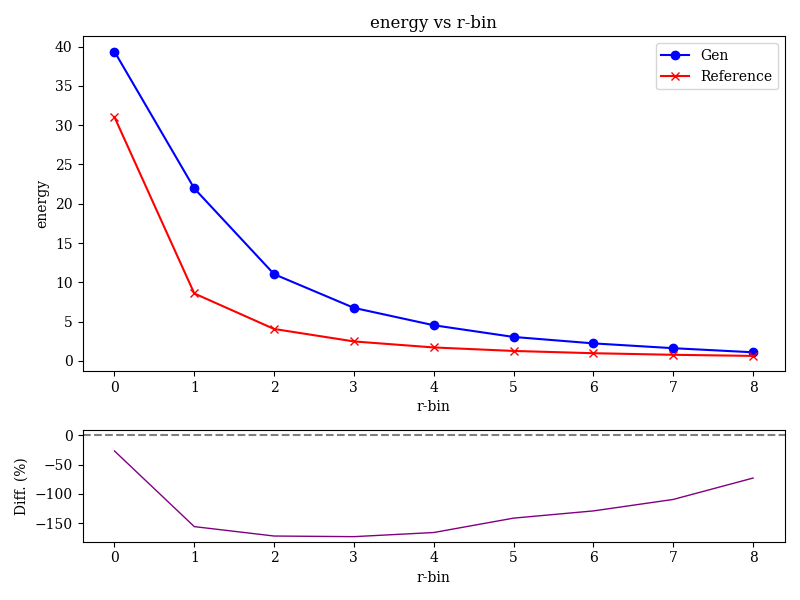
\includegraphics[width=\textwidth]{Figures/a1_2.png}
        \caption{Energy vs Radius}
        \label{fig:a1-2}
    \end{subfigure}
    \hfill
    \begin{subfigure}[b]{0.23\textwidth}
        \centering
        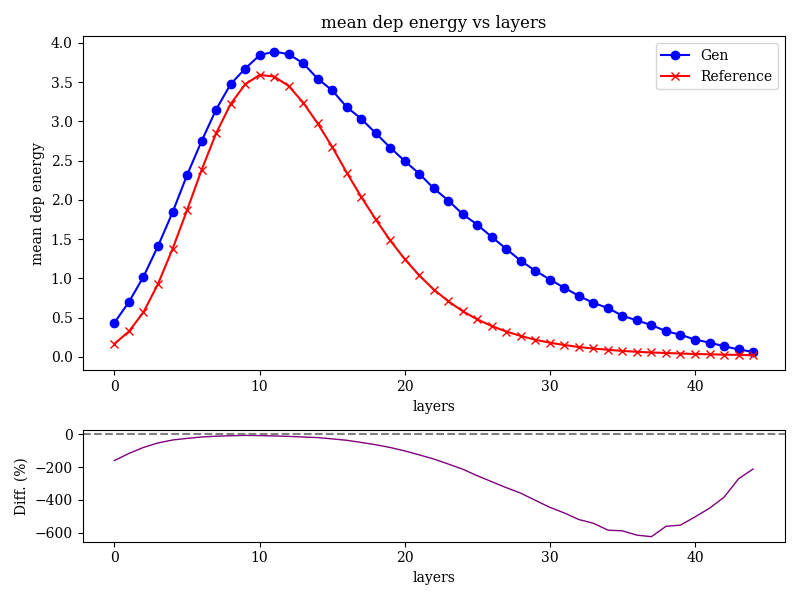
\includegraphics[width=\textwidth]{Figures/a1_3.png}
        \caption{Energy vs Z}
        \label{fig:a1-3}
    \end{subfigure}
    \hfill
    \begin{subfigure}[b]{0.23\textwidth}
        \centering
        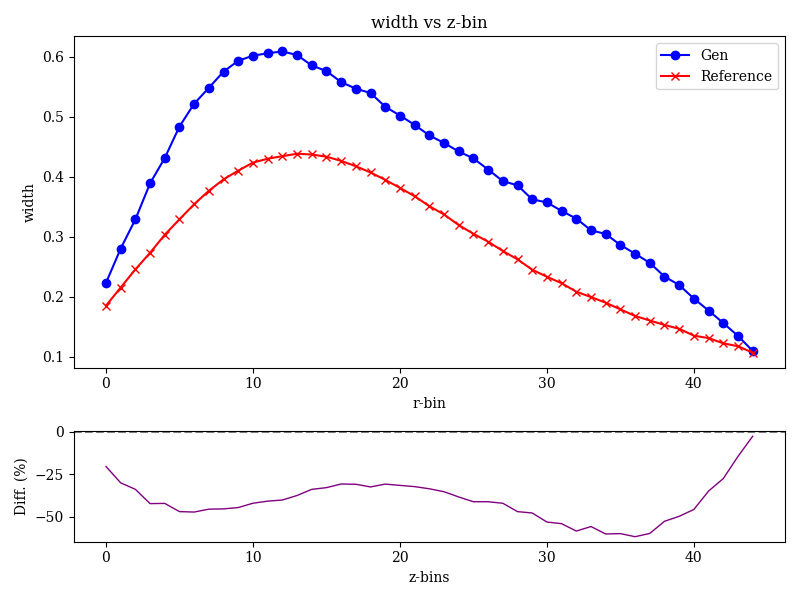
\includegraphics[width=\textwidth]{Figures/a1_4.png}
        \caption{R-width vs Layers}
        \label{fig:a1-4}
    \end{subfigure}
    \hfill
    \begin{subfigure}[b]{0.23\textwidth}  % Adjust width to fit 4 figures
        \centering
        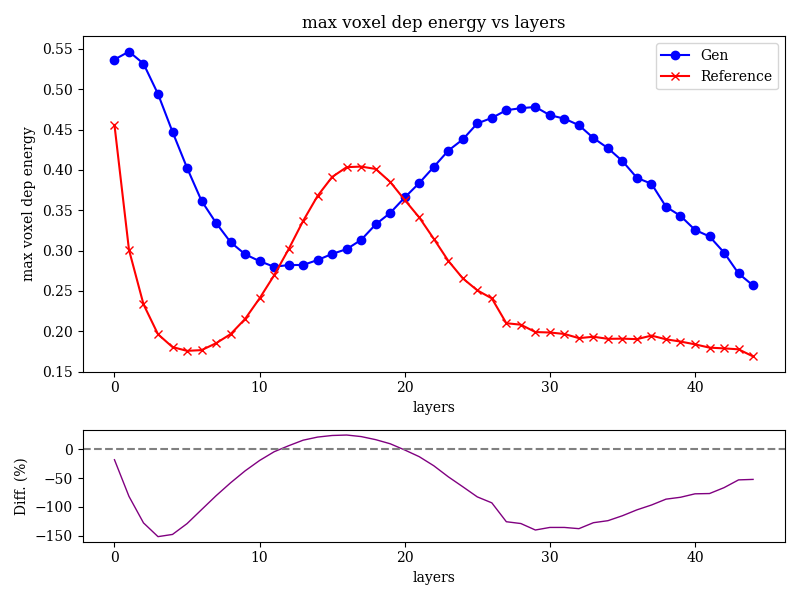
\includegraphics
        [width=\textwidth]{Figures/a1_5.png}
        \caption{Max Voxel Deposit vs Layers}
        
        \label{fig:a1-1}
    \end{subfigure}
    
    \vspace{0.6cm} % Space between rows

    % Second row: 3 figures
    \begin{subfigure}[b]{0.3\textwidth}  % Adjust width to fit 3 figures
        \centering
        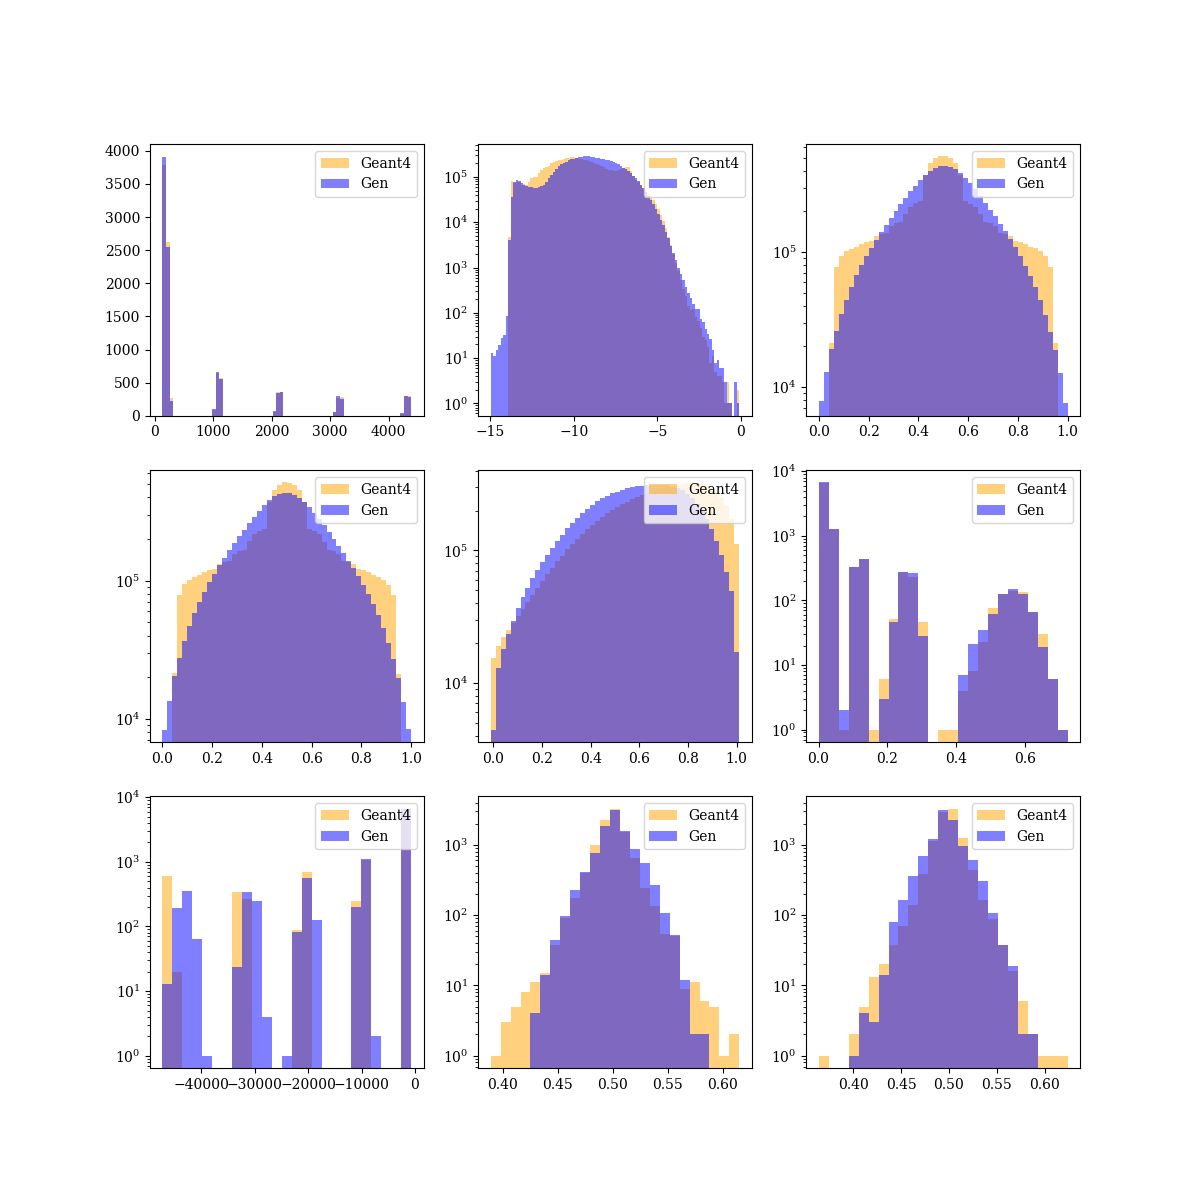
\includegraphics
        [width=\textwidth]{Figures/a1-1.png}
        \caption{1D Histogram}
        \label{fig:a1-5}
    \end{subfigure}
    \hfill
    \begin{subfigure}[b]{0.3\textwidth}
        \centering
        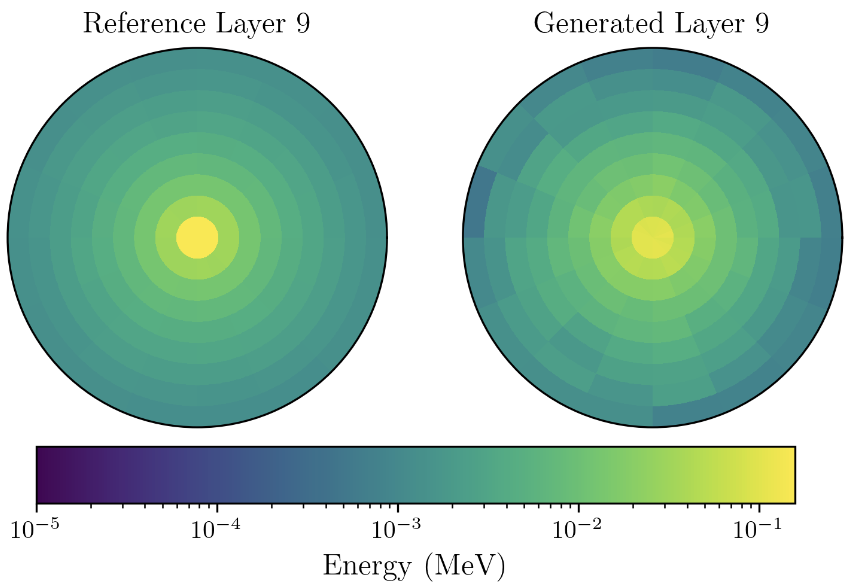
\includegraphics[width=\textwidth]{Figures/comparison.png}
        \caption{Energy voxel comparison}
        \label{fig:a1_5}
    \end{subfigure}
    \hfill
    \begin{subfigure}[b]{0.3\textwidth}
        \centering
        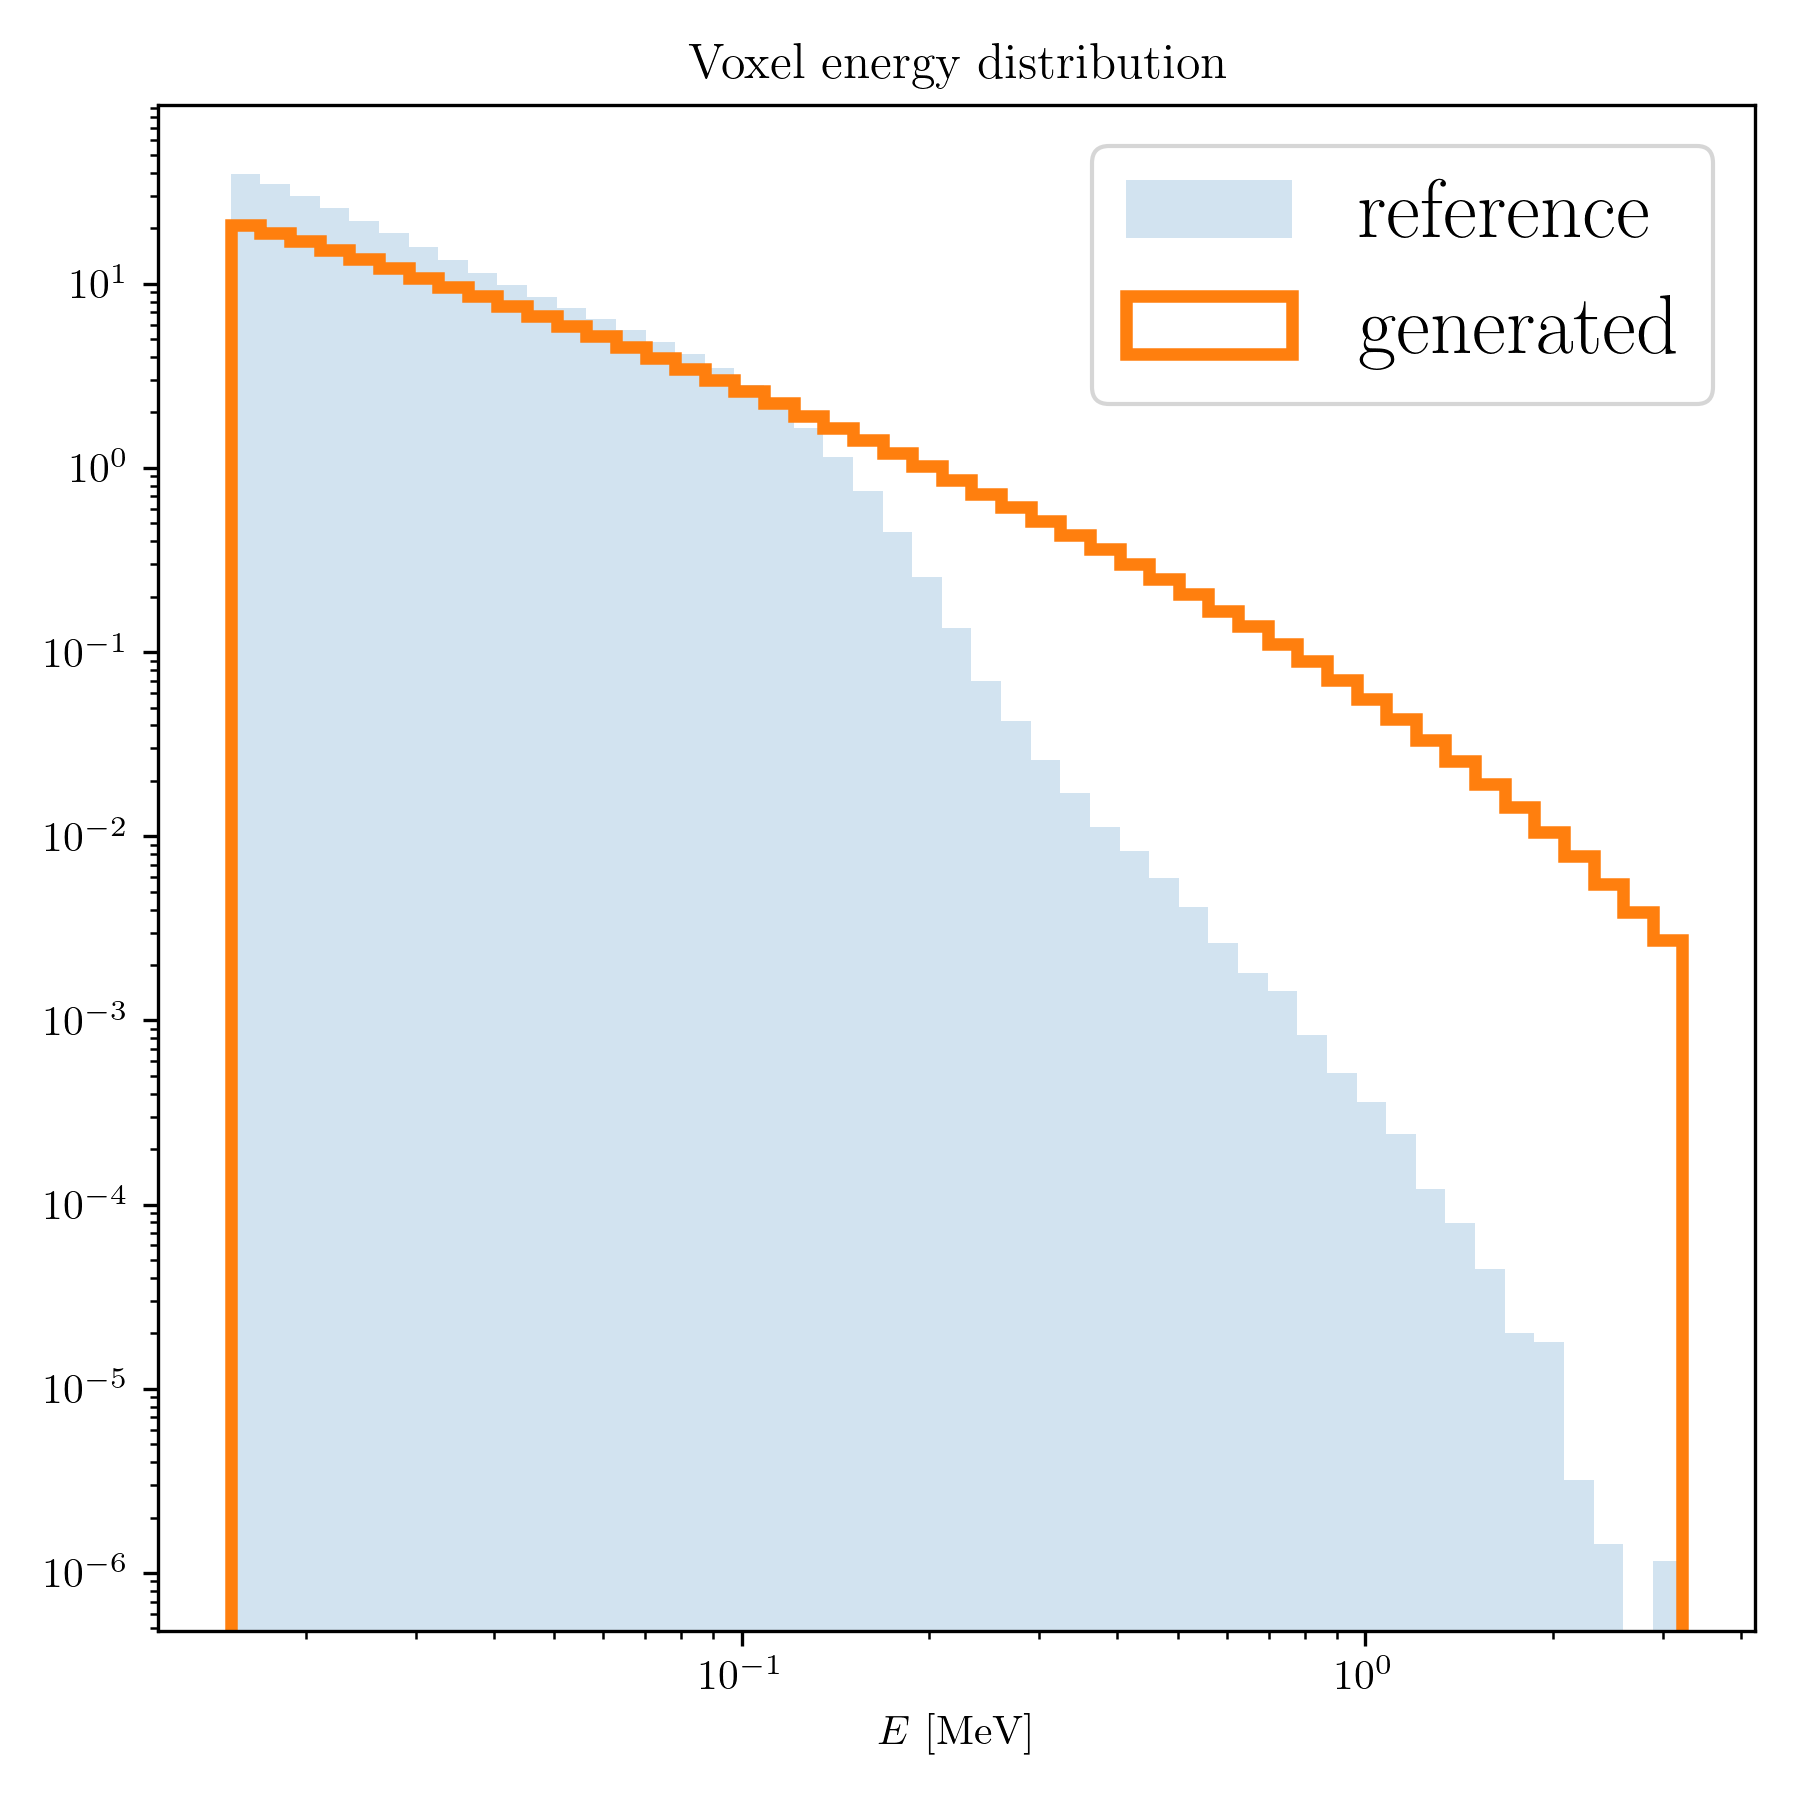
\includegraphics[width=\textwidth]{Figures/a1_7.png}
        \caption{Energy Deposit}
        \label{fig:a1_7}
    \end{subfigure}
\end{figure}

\newpage
\section{Best Result for Single Bucket Data}


\begin{figure}[htbp]
    \centering
    % First row: 4 figures
    \begin{subfigure}[b]{0.23\textwidth}
        \centering
        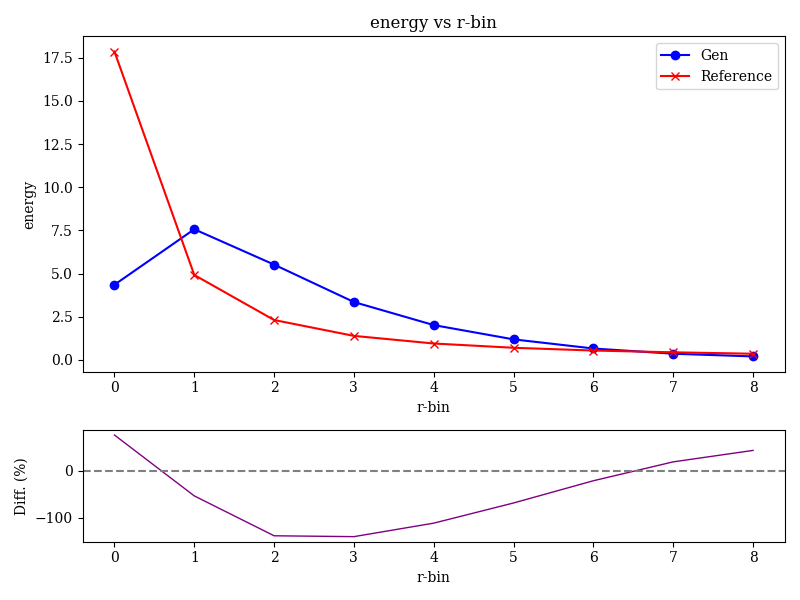
\includegraphics[width=\textwidth]{Figures/2_2.png}
        \caption{Energy vs Radius}
        \label{fig:a2_2}
    \end{subfigure}
    \hfill
    \begin{subfigure}[b]{0.23\textwidth}
        \centering
        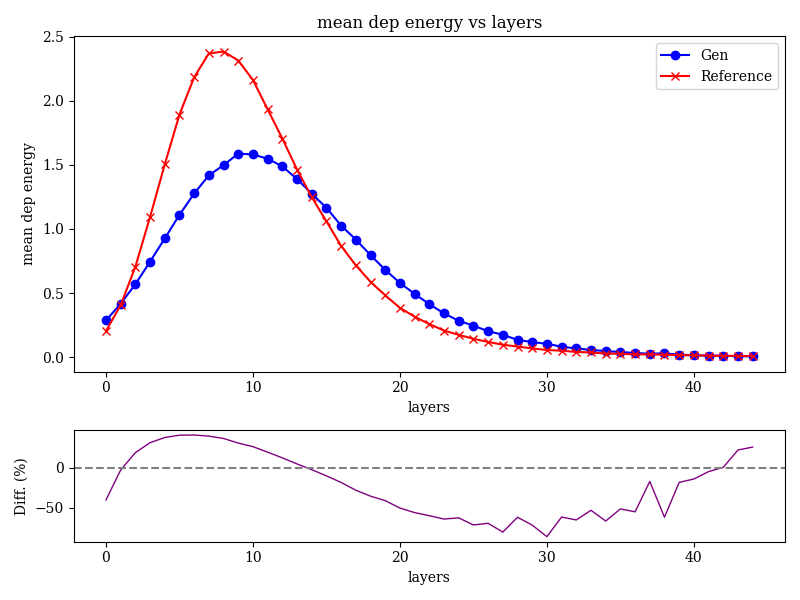
\includegraphics[width=\textwidth]{Figures/2_3.png}
        \caption{Energy vs Z}
        \label{fig:a2_3}
    \end{subfigure}
    \hfill
    \begin{subfigure}[b]{0.23\textwidth}
        \centering
        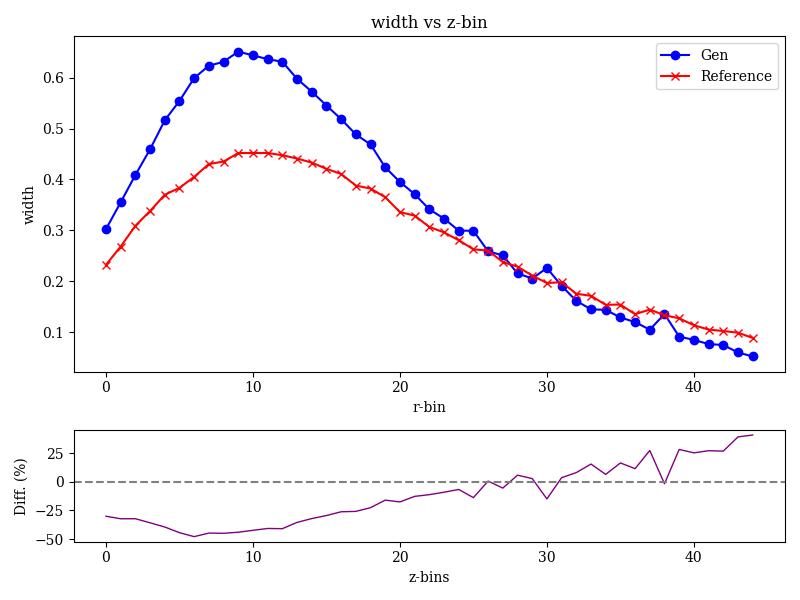
\includegraphics[width=\textwidth]{Figures/2_4.png}
        \caption{R-width vs layers}
        \label{fig:a2_4}
    \end{subfigure}
    \hfill
    \begin{subfigure}[b]{0.23\textwidth}  % Adjust width to fit 4 figures
        \centering
        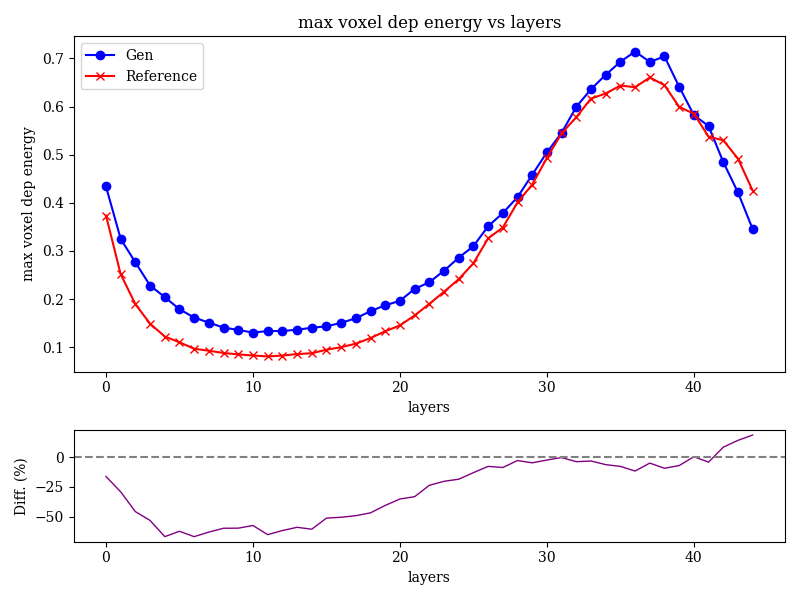
\includegraphics
        [width=\textwidth]{Figures/2_5.png}
        \caption{Max Voxel Deposit vs Layers}
        \label{fig:a2_1}
    \end{subfigure}

    \vspace{0.6cm} % Space between rows

    % Second row: 3 figures
    \begin{subfigure}[b]{0.3\textwidth}  % Adjust width to fit 3 figures
        \centering
        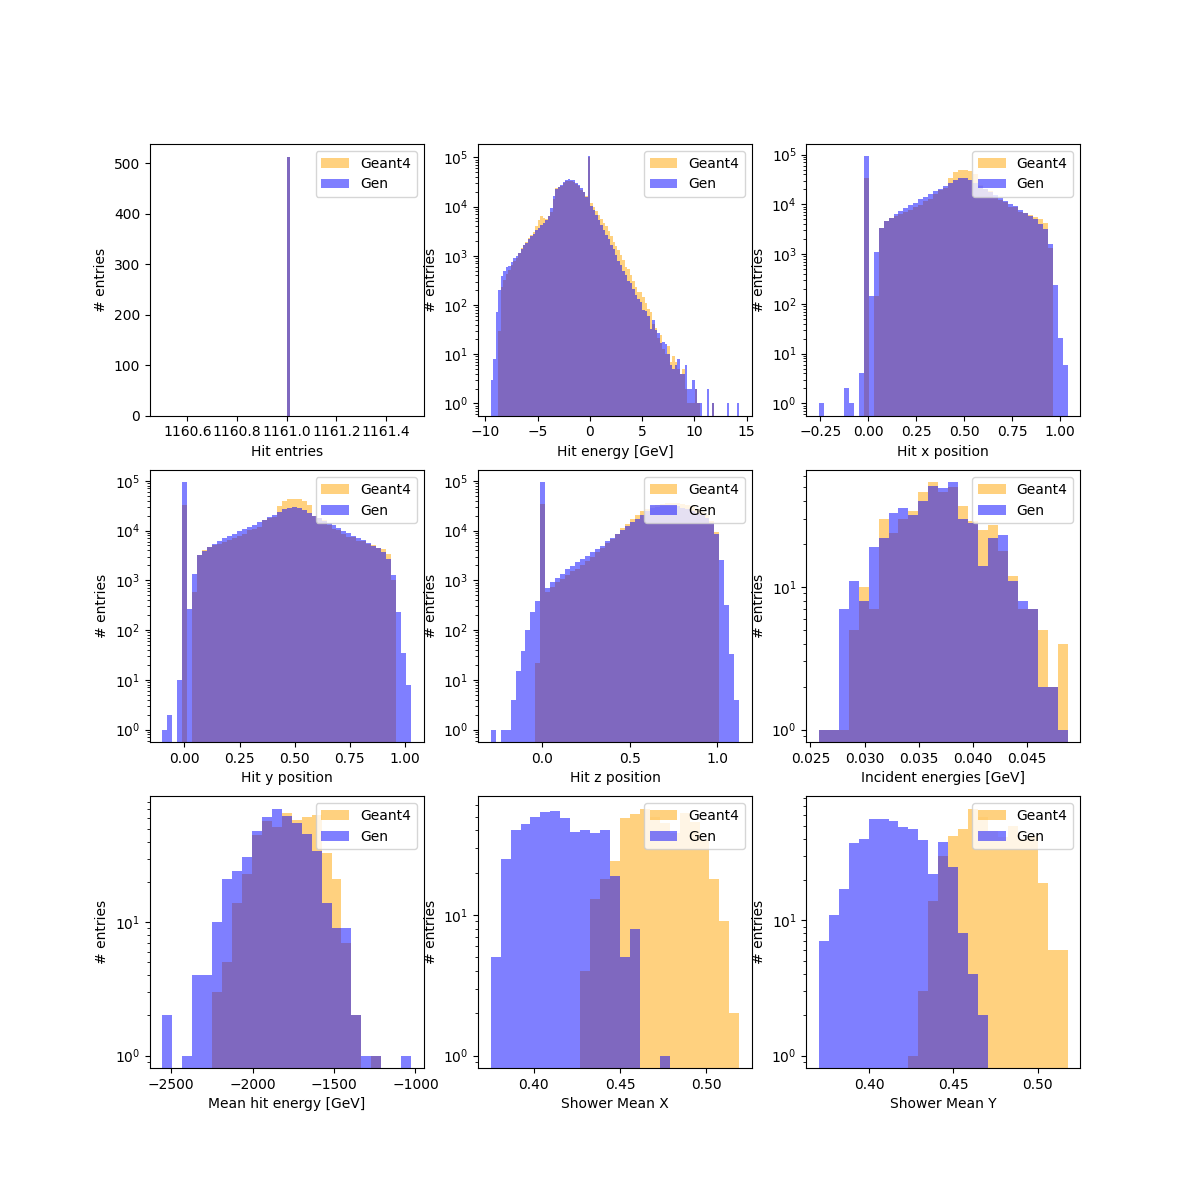
\includegraphics
        [width=\textwidth]{Figures/a2_1.png}
        \caption{1D Histogram}
        \label{fig:a2_5}
    \end{subfigure}
    \hfill
    \begin{subfigure}[b]{0.3\textwidth}
        \centering
        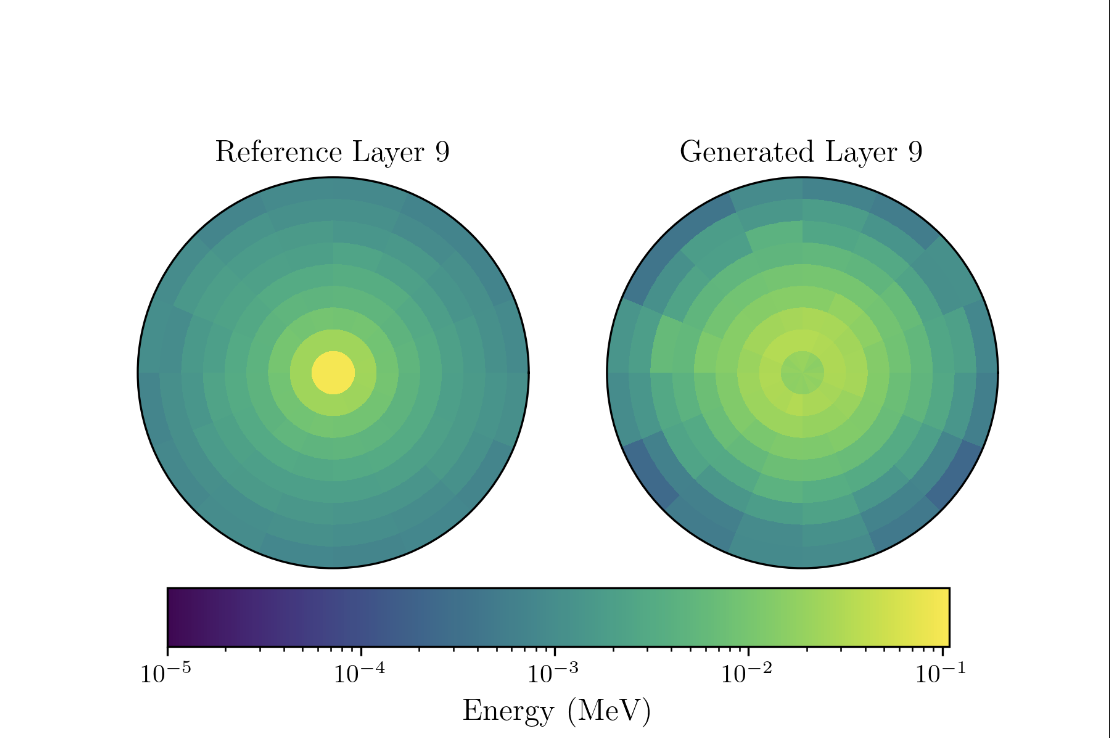
\includegraphics[width=\textwidth]{Figures/a2_5.png}
        \caption{Energy voxel comparison}
        \label{fig:a2_6}
    \end{subfigure}
    \hfill
    \begin{subfigure}[b]{0.3\textwidth}
        \centering
        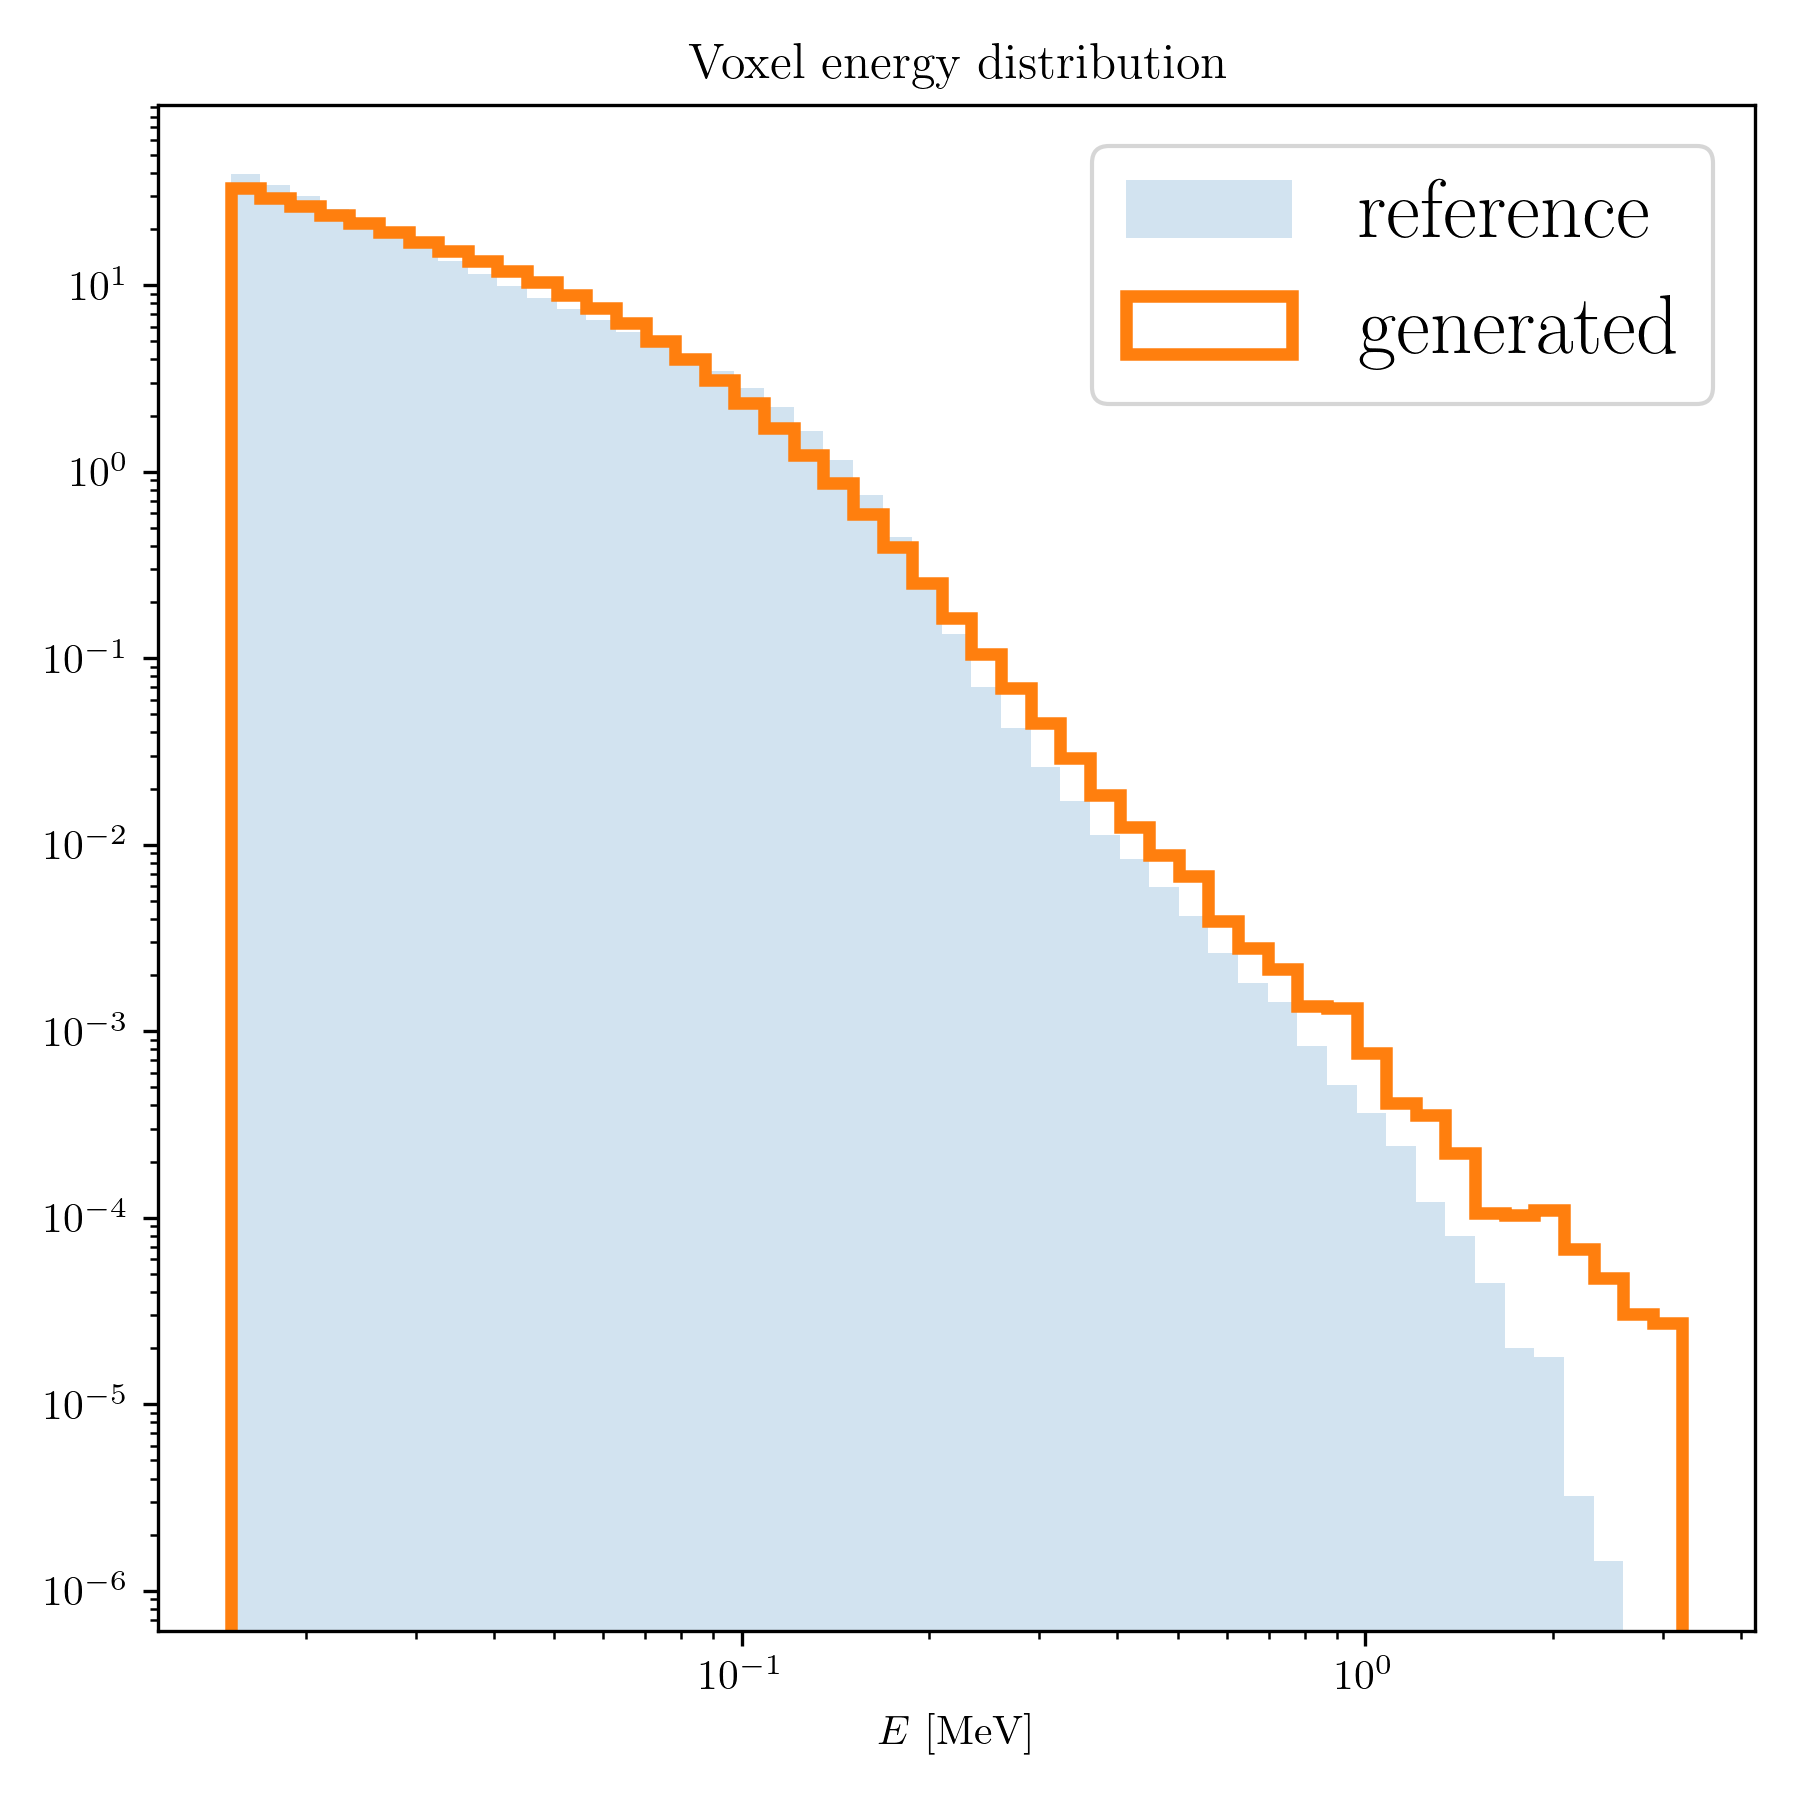
\includegraphics[width=\textwidth]{Figures/a2_6.png}
        \caption{Energy Deposit}
        \label{fig:a2_7}
    \end{subfigure}
\end{figure}
% \section{Result for without using incident energy}
% 7 pictures in total
\newpage
\section{Result for using different Preprocessor}


\begin{figure}[htbp]
    \centering
    % First row: 4 figures
    \begin{subfigure}[b]{0.3\textwidth}
        \centering
        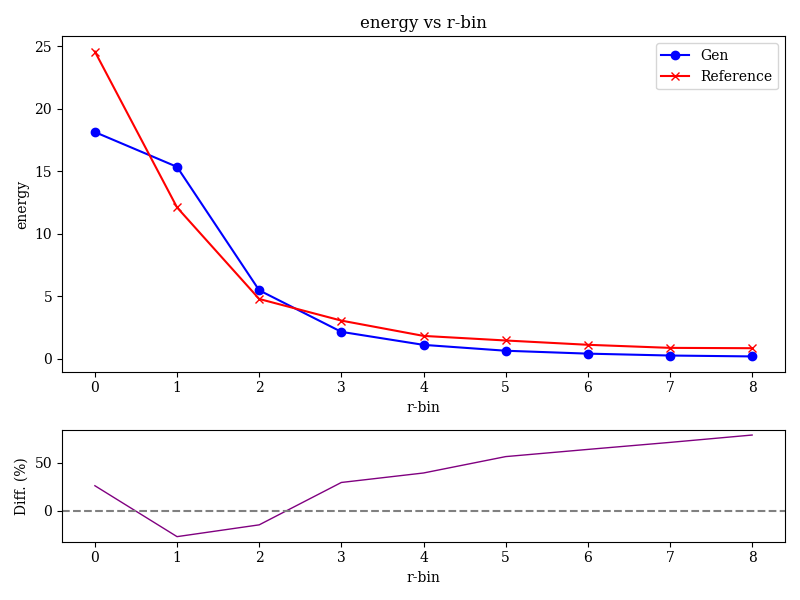
\includegraphics[width=\textwidth]{Figures/robust2.png}
        \caption{Energy vs Radius}
        \label{fig:robust2}
    \end{subfigure}
    \hfill
    \begin{subfigure}[b]{0.3\textwidth}
        \centering
        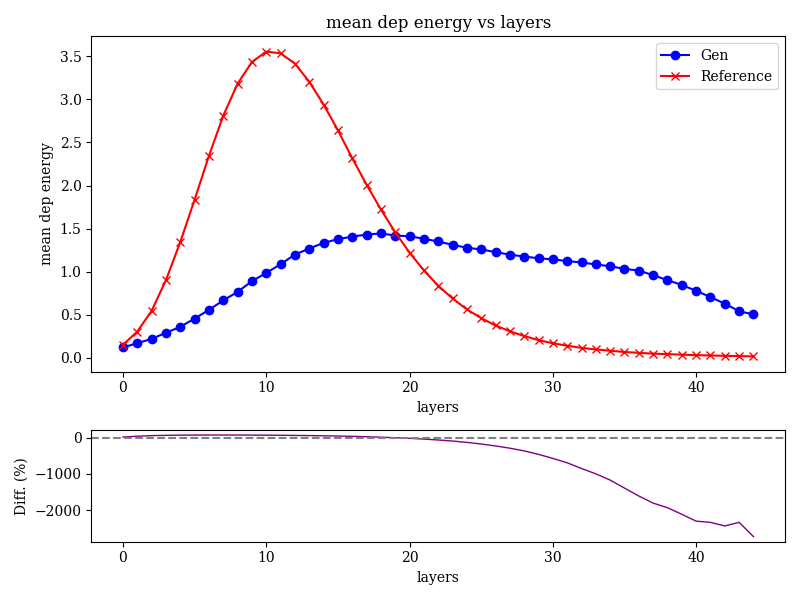
\includegraphics[width=\textwidth]{Figures/robust3.png}
        \caption{Energy vs Z}
        \label{fig:robust3}
    \end{subfigure}
    \hfill
    \begin{subfigure}[b]{0.3\textwidth}
        \centering
        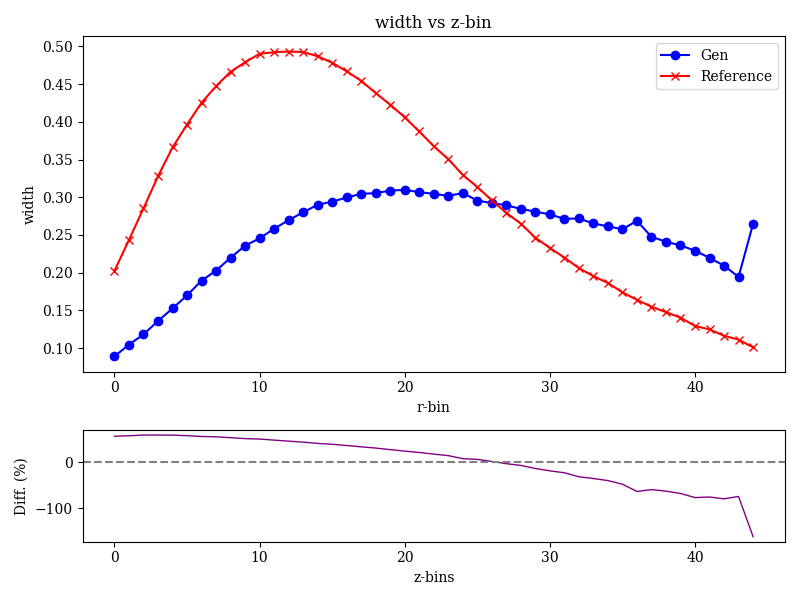
\includegraphics[width=\textwidth]{Figures/robust4.png}
        \caption{R-width vs layers}
        \label{fig:robust4}
    \end{subfigure}
    

    \vspace{0.35cm} % Space between rows

    % Second row: 3 figures
    
    \begin{subfigure}[b]{0.3\textwidth}  % Adjust width to fit 4 figures
        \centering
        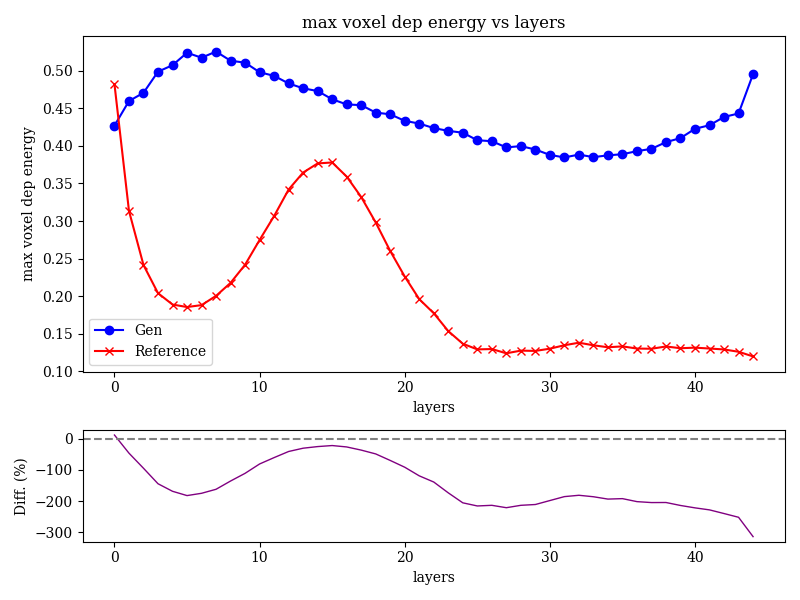
\includegraphics
        [width=\textwidth]{Figures/robust5.png}
        \caption{Max Voxel Deposit vs Layers}
        \label{fig:robust5}
    \end{subfigure}
    \hfill
    \begin{subfigure}[b]{0.3\textwidth}  % Adjust width to fit 3 figures
        \centering
        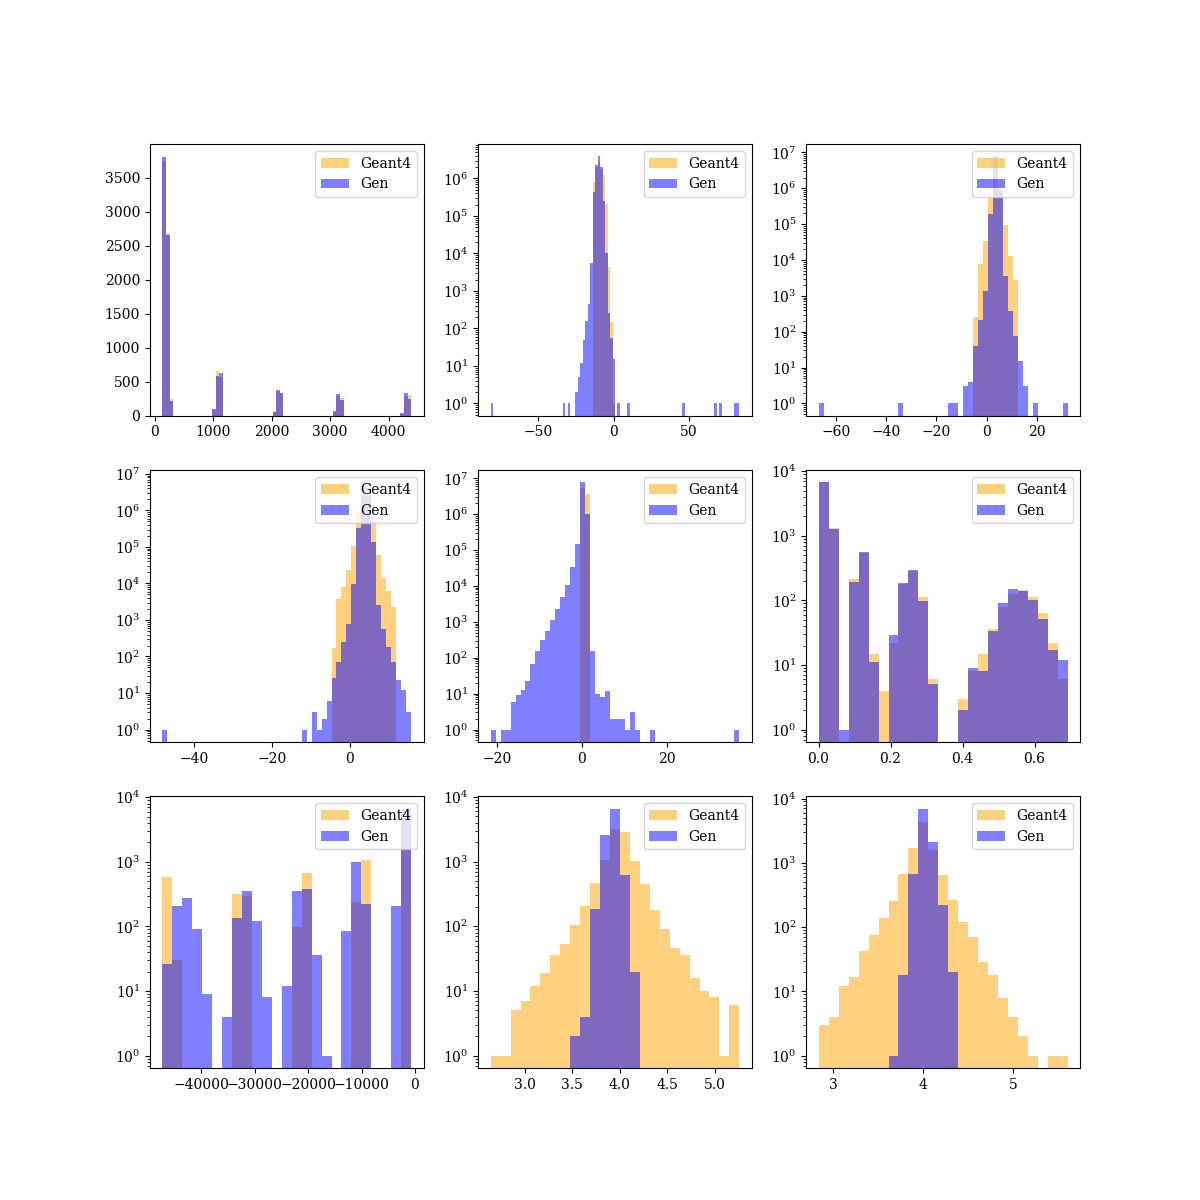
\includegraphics
        [width=\textwidth]{Figures/robust1.png}
        \caption{1D Histogram}
        \label{fig:robust1}
    \end{subfigure}
    \hfill
    \begin{subfigure}[b]{0.3\textwidth}
        \centering
        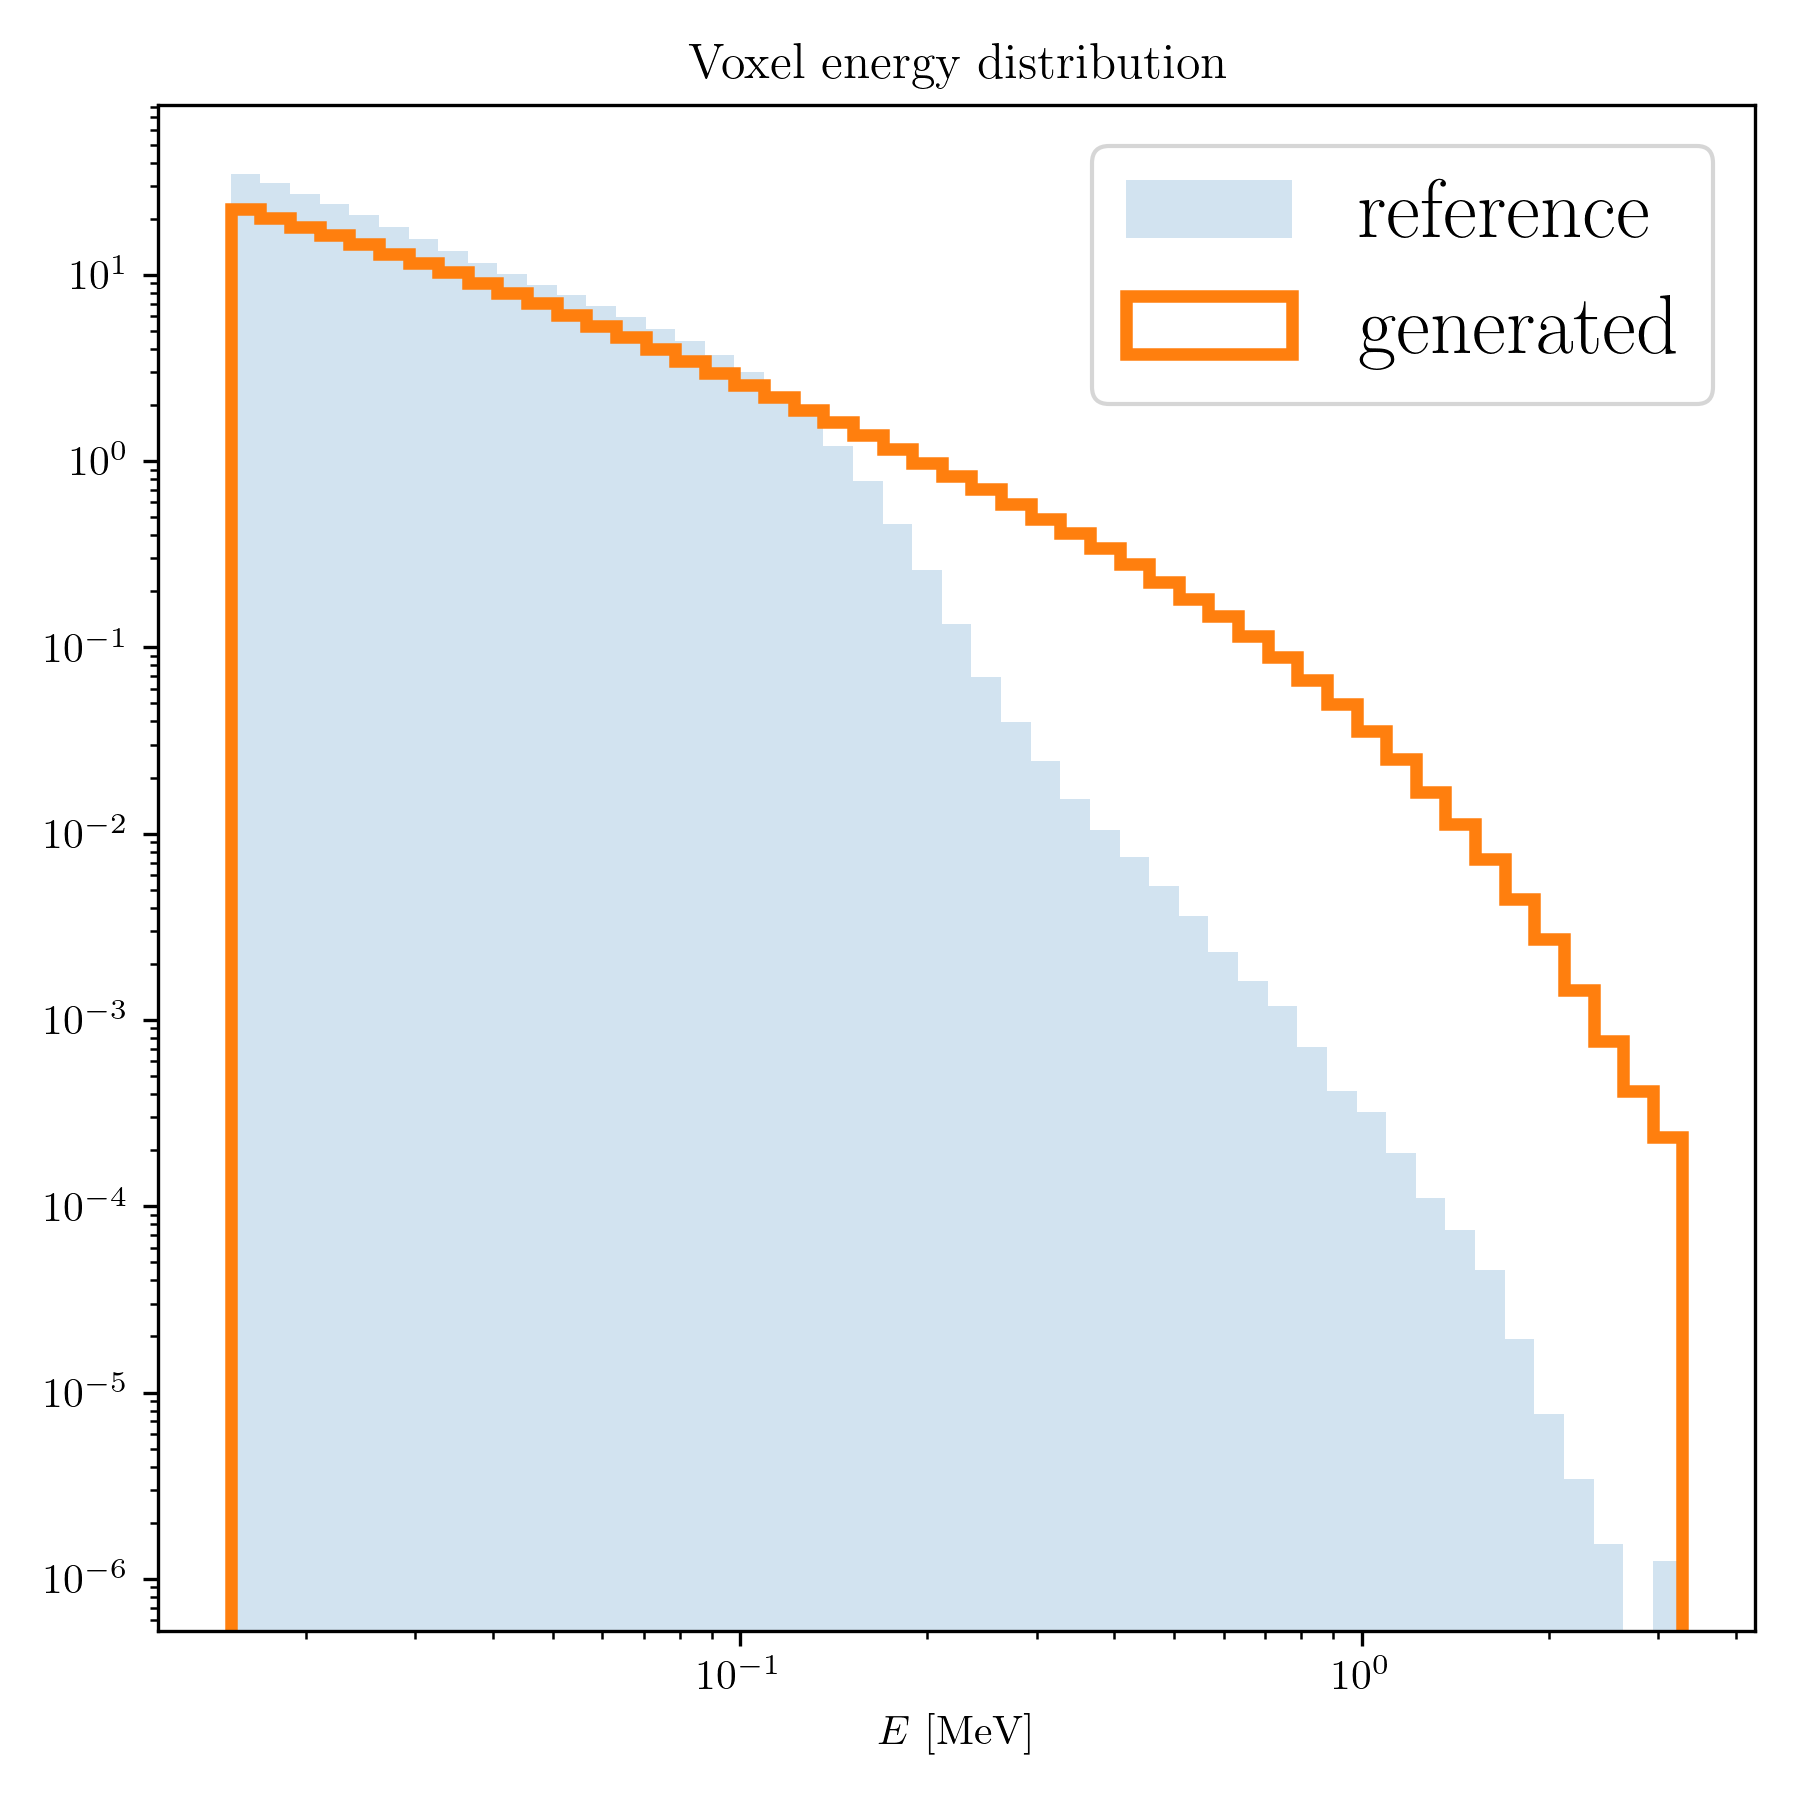
\includegraphics[width=\textwidth]{Figures/robust6.png}
        \caption{Energy Deposit}
        \label{fig:robust6}
    \end{subfigure}
    \caption{Result for using robust preprocessor}
\end{figure}

\begin{figure}
    \centering
    % First row: 4 figures
    \begin{subfigure}[b]{0.3\textwidth}
        \centering
        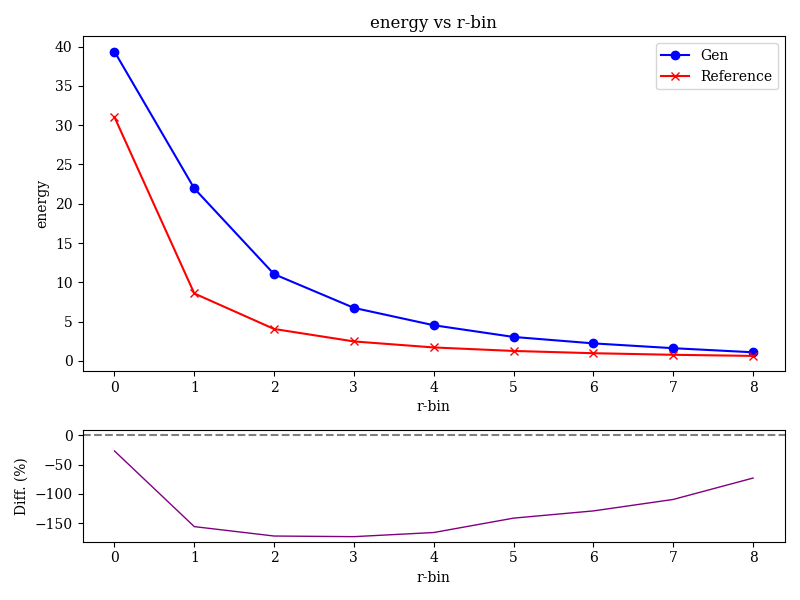
\includegraphics[width=\textwidth]{Figures/quantile2.png}
        \caption{Energy vs Radius}
        \label{fig:quantile2}
    \end{subfigure}
    \hfill
    \begin{subfigure}[b]{0.3\textwidth}
        \centering
        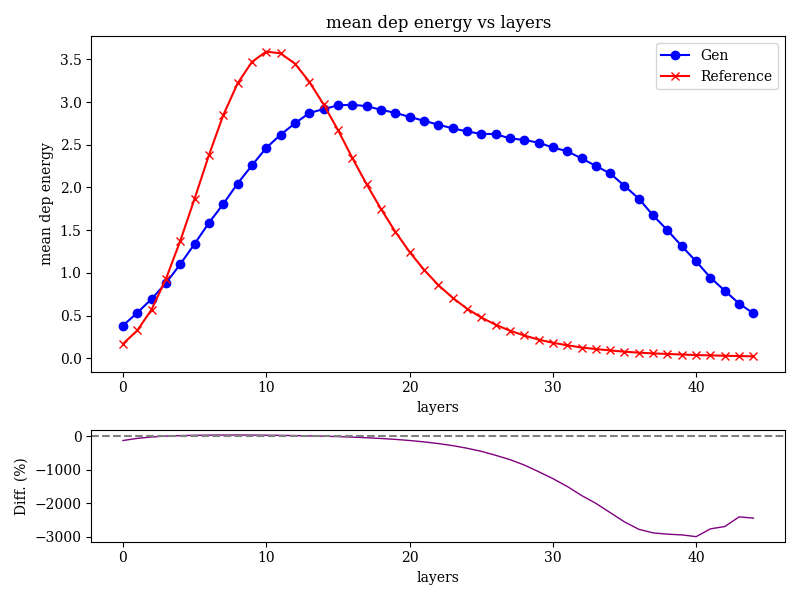
\includegraphics[width=\textwidth]{Figures/quantile3.png}
        \caption{Energy vs Z}
        \label{fig:quantile3}
    \end{subfigure}
    \hfill
    \begin{subfigure}[b]{0.3\textwidth}
        \centering
        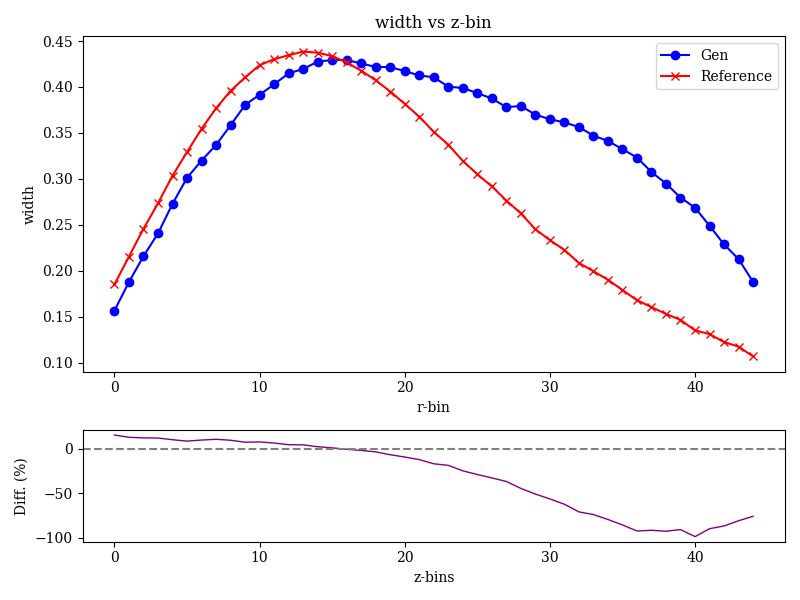
\includegraphics[width=\textwidth]{Figures/quantile4.png}
        \caption{R-width vs layers}
        \label{fig:quantile4}
    \end{subfigure}
    

    \vspace{0.35cm} % Space between rows

    % Second row: 3 figures
    
    \begin{subfigure}[b]{0.3\textwidth}  % Adjust width to fit 4 figures
        \centering
        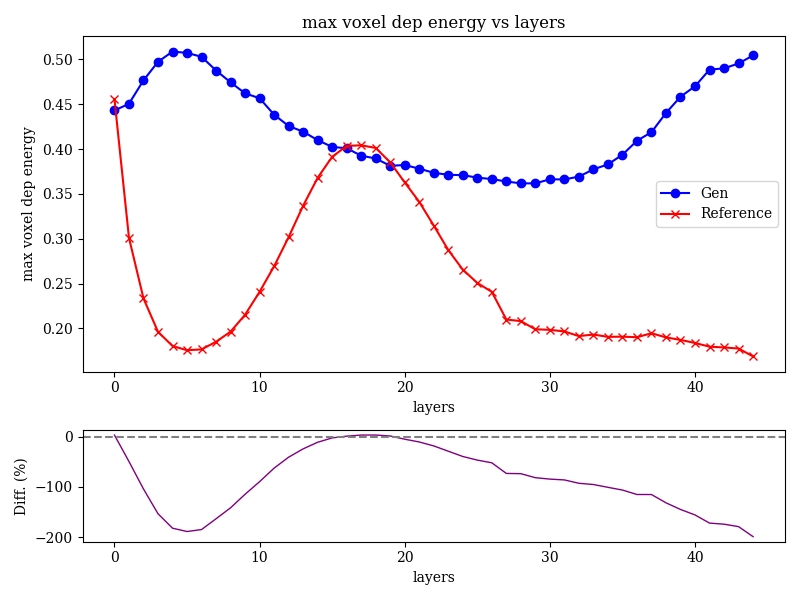
\includegraphics
        [width=\textwidth]{Figures/quantile5.png}
        \caption{Max Voxel Deposit vs Layers}
        \label{fig:quantile5}
    \end{subfigure}
    \hfill
    \begin{subfigure}[b]{0.3\textwidth}  % Adjust width to fit 3 figures
        \centering
        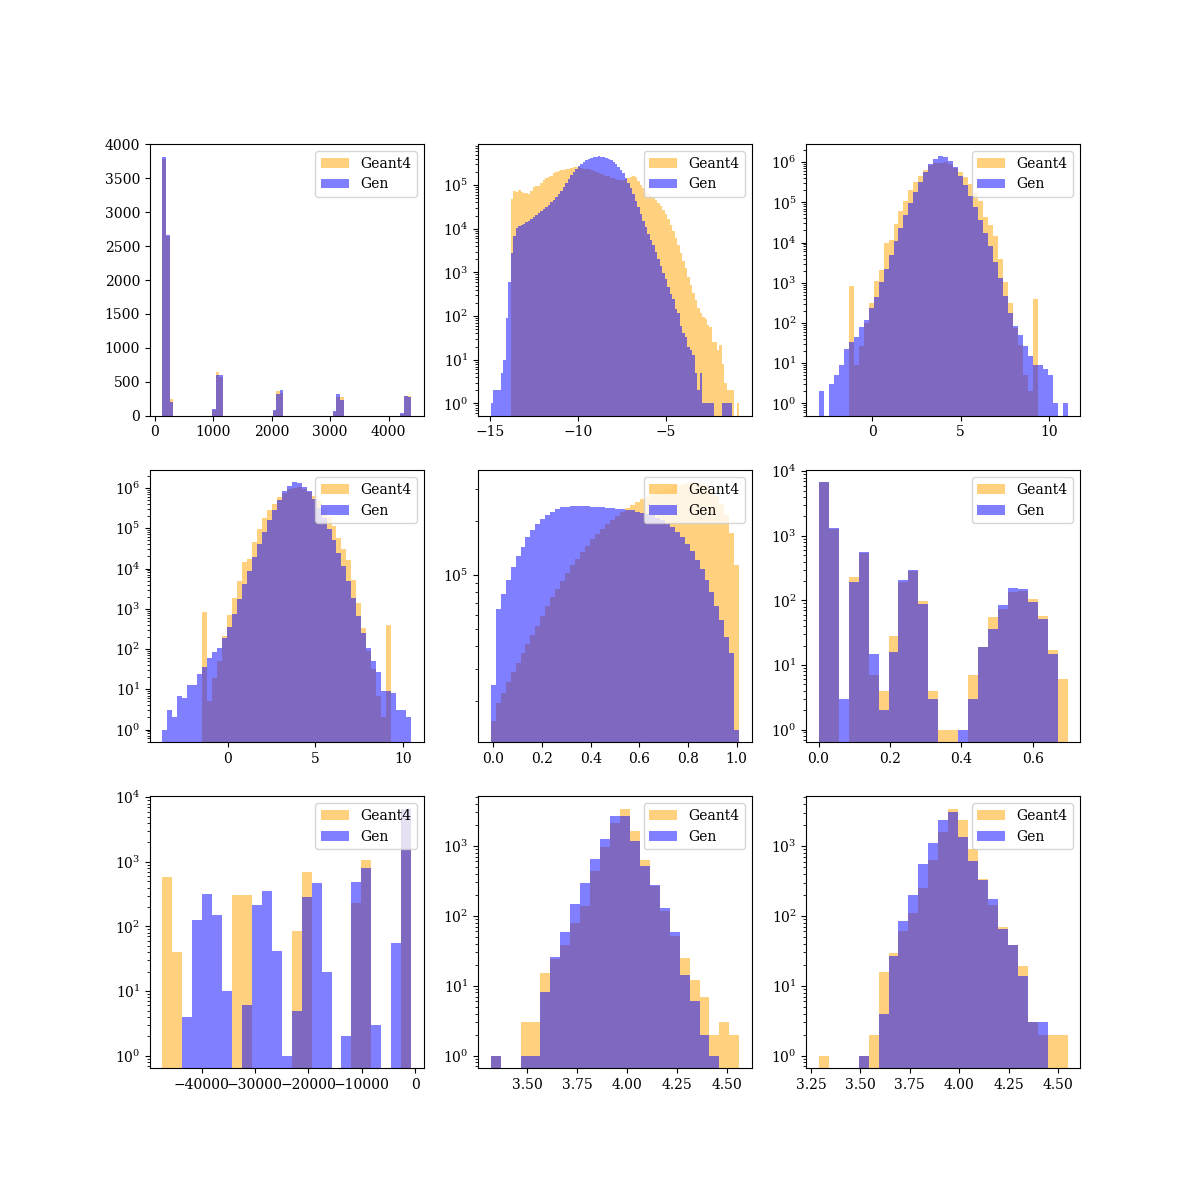
\includegraphics
        [width=\textwidth]{Figures/quantile1.png}
        \caption{1D Histogram}
        \label{fig:quantile1}
    \end{subfigure}
    \hfill
    \begin{subfigure}[b]{0.3\textwidth}
        \centering
        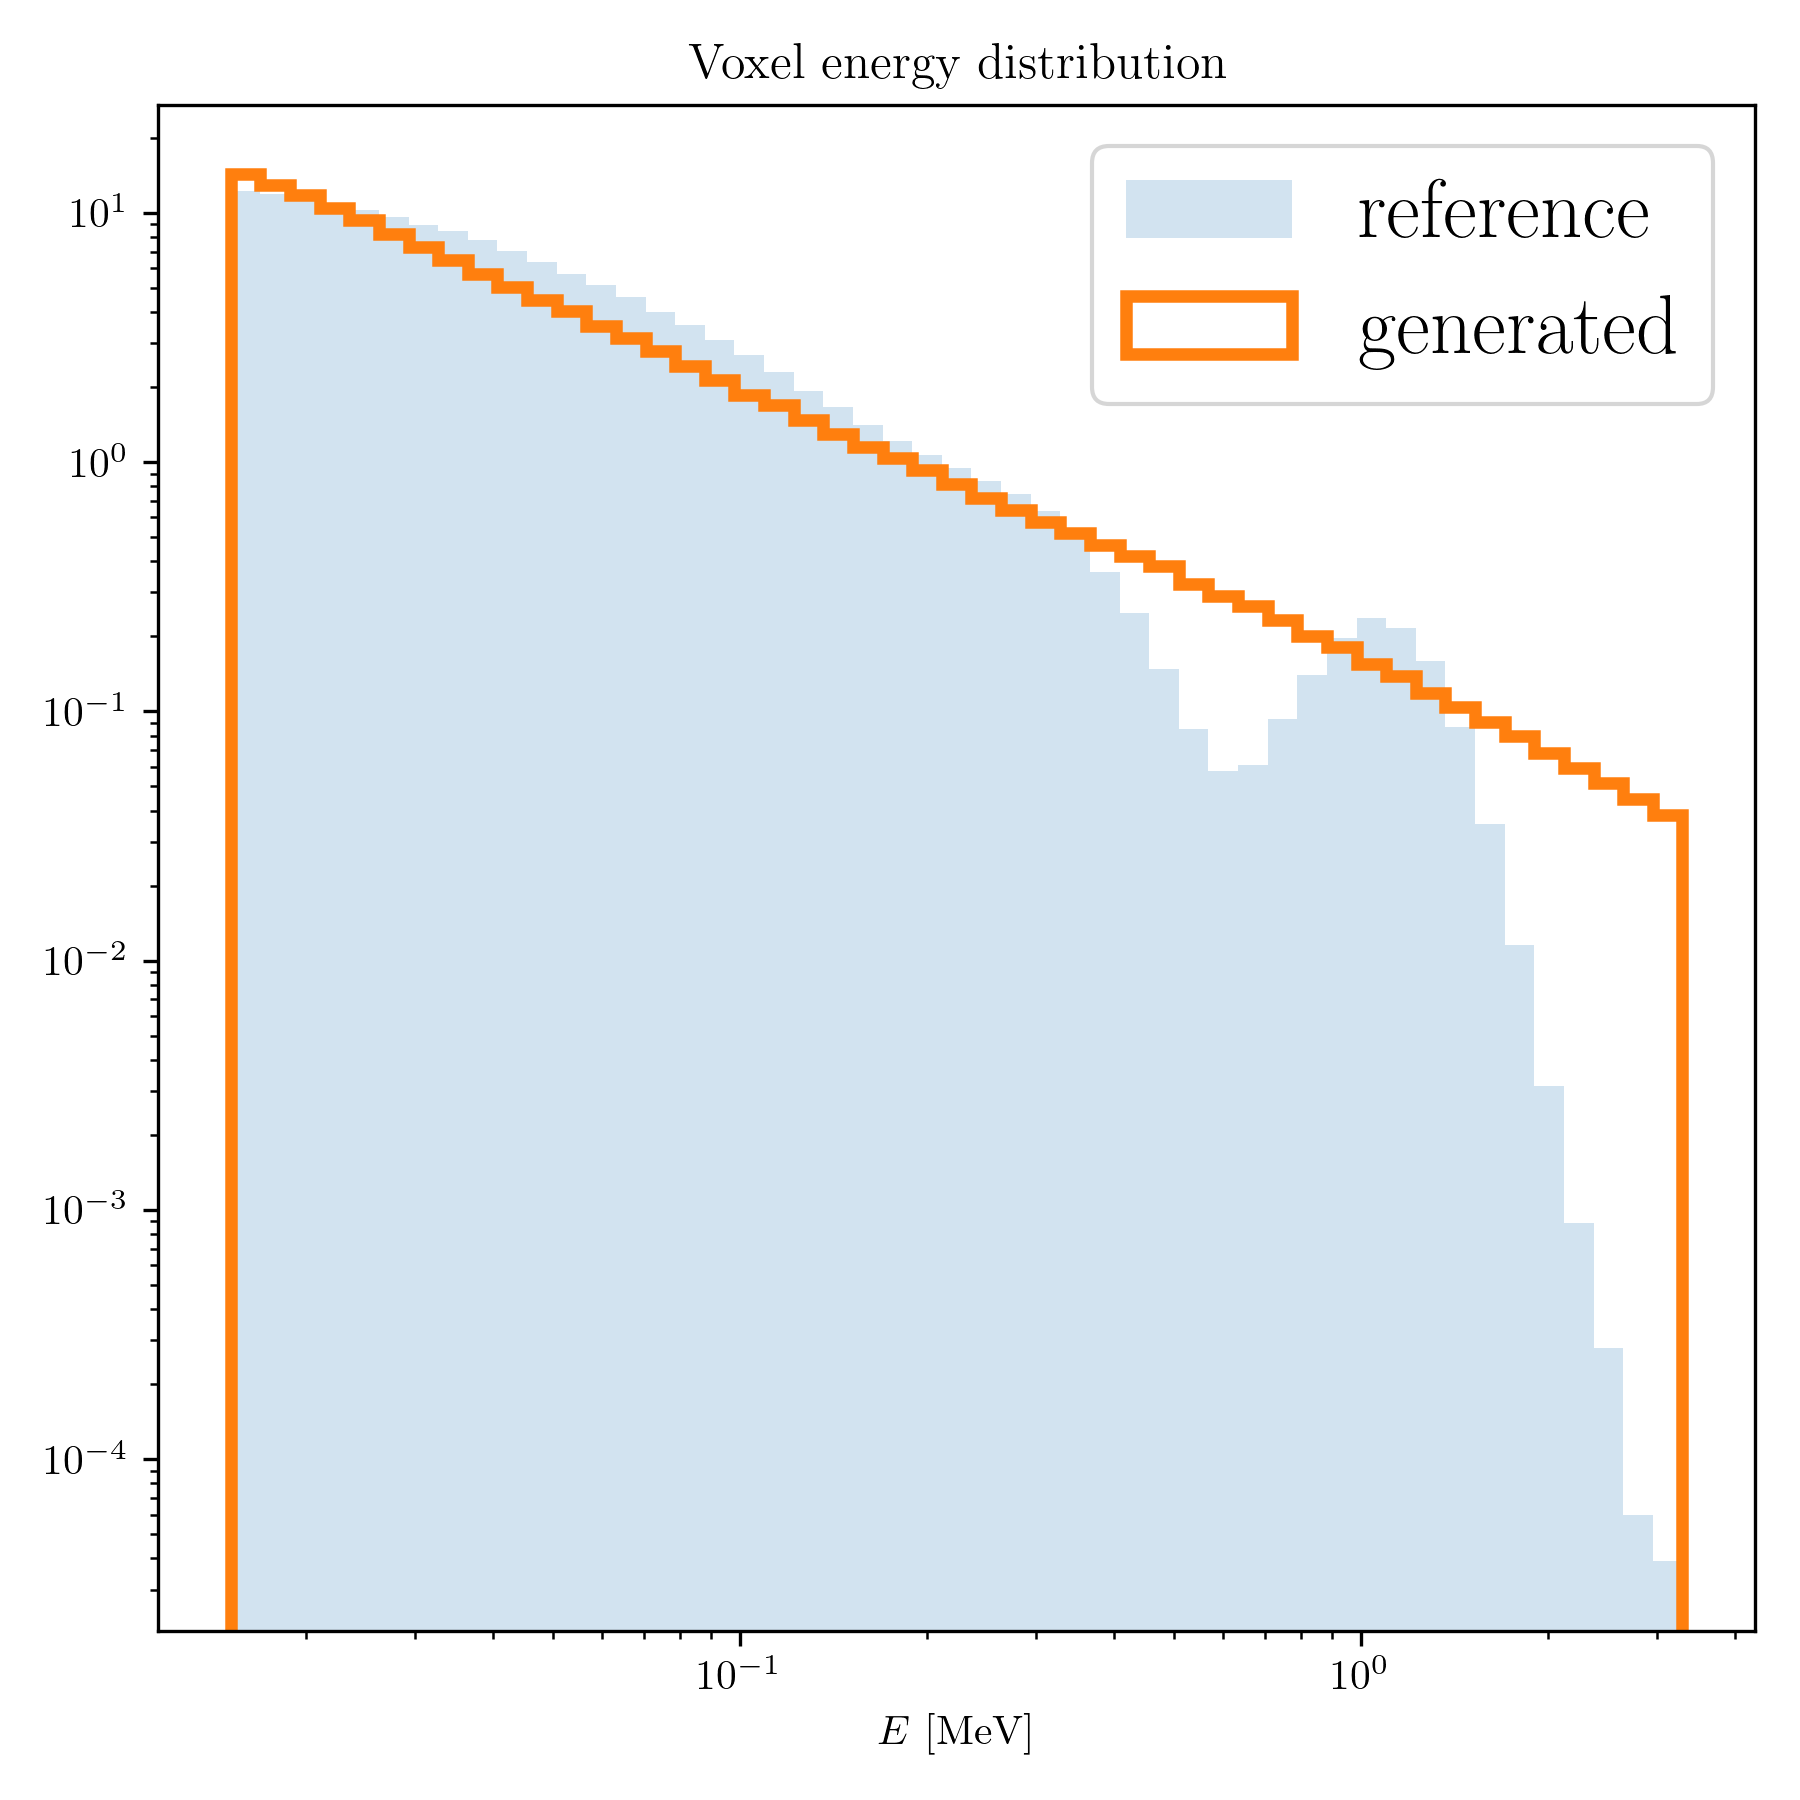
\includegraphics[width=\textwidth]{Figures/quantile6.png}
        \caption{Energy Deposit}
        \label{fig:quantile6}
    \end{subfigure}
    \caption{Result for using quantile preprocessor}
\end{figure}

\begin{figure}
    \centering
    % First row: 4 figures
    \begin{subfigure}[b]{0.3\textwidth}
        \centering
        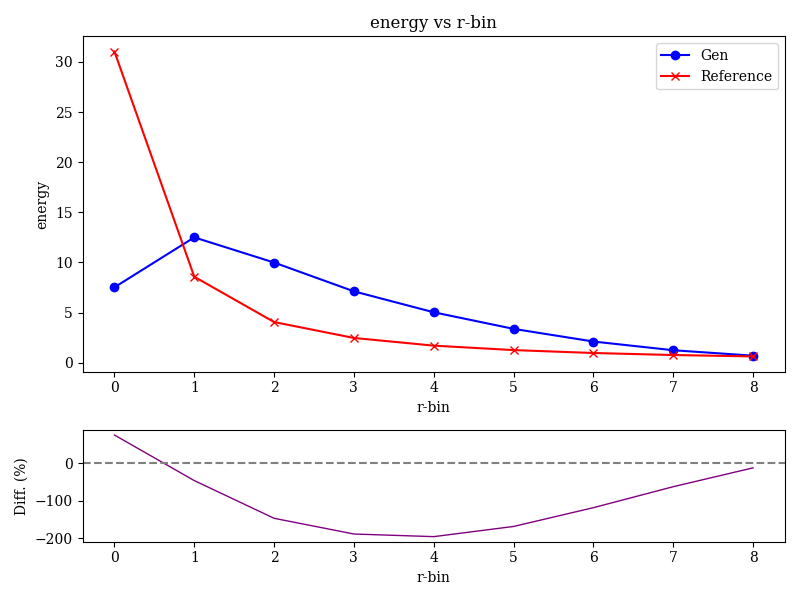
\includegraphics[width=\textwidth]{Figures/exponential2.png}
        \caption{Energy vs Radius}
        \label{fig:exp2}
    \end{subfigure}
    \hfill
    \begin{subfigure}[b]{0.3\textwidth}
        \centering
        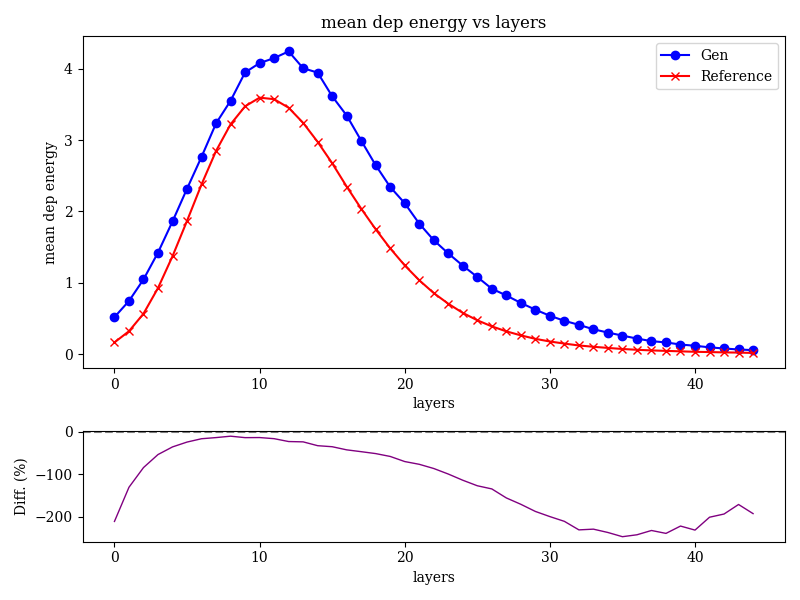
\includegraphics[width=\textwidth]{Figures/exponential3.png}
        \caption{Energy vs Z}
        \label{fig:exp3}
    \end{subfigure}
    \hfill
    \begin{subfigure}[b]{0.3\textwidth}
        \centering
        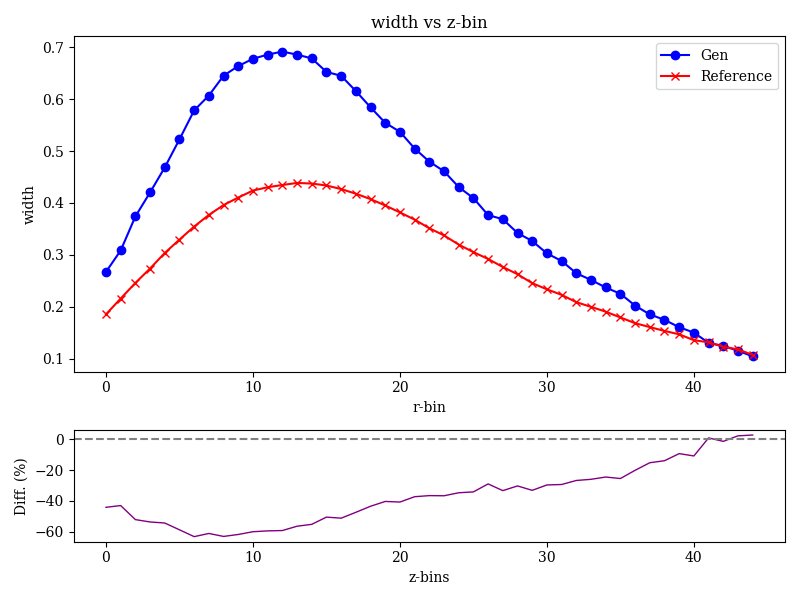
\includegraphics[width=\textwidth]{Figures/exponential4.png}
        \caption{R-width vs layers}
        \label{fig:exp4}
    \end{subfigure}
    

    \vspace{0.35cm} % Space between rows

    % Second row: 3 figures
    
    \begin{subfigure}[b]{0.3\textwidth}  % Adjust width to fit 4 figures
        \centering
        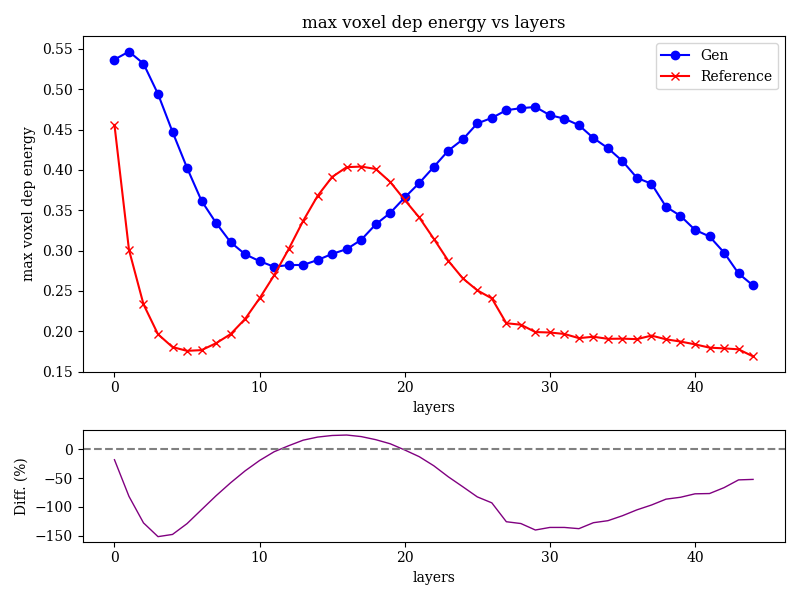
\includegraphics
        [width=\textwidth]{Figures/a1_5.png}
        \caption{Max Voxel Deposit vs Layers}
        \label{fig:exp5}
    \end{subfigure}
    \hfill
    \begin{subfigure}[b]{0.3\textwidth}  % Adjust width to fit 3 figures
        \centering
        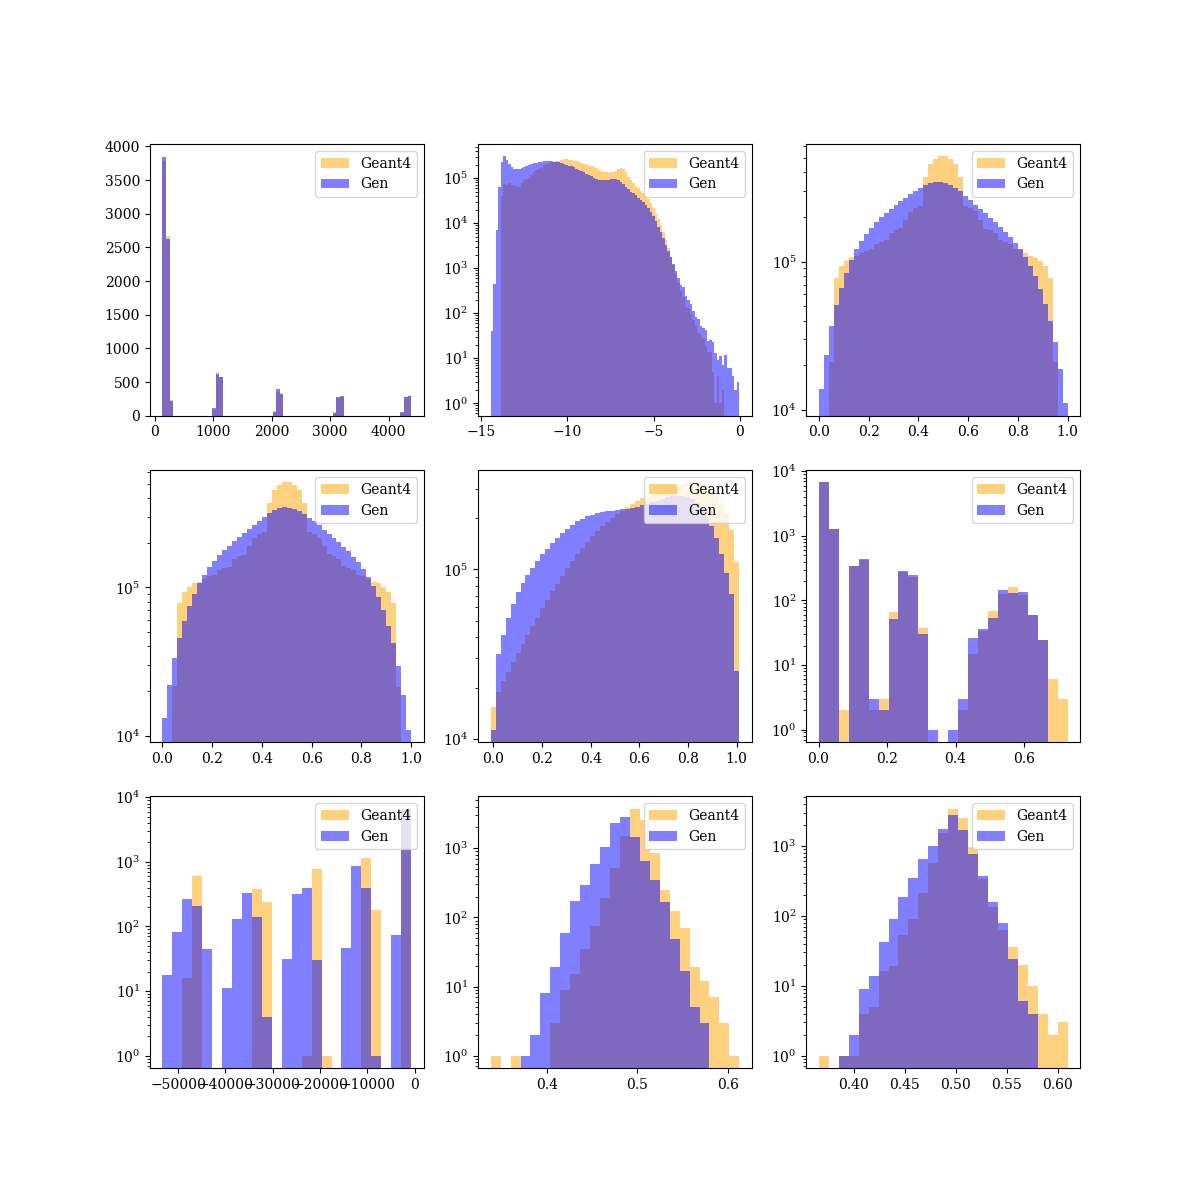
\includegraphics
        [width=\textwidth]{Figures/exponential1.png}
        \caption{1D Histogram}
        \label{fig:exp1}
    \end{subfigure}
    \hfill
    \begin{subfigure}[b]{0.3\textwidth}
        \centering
        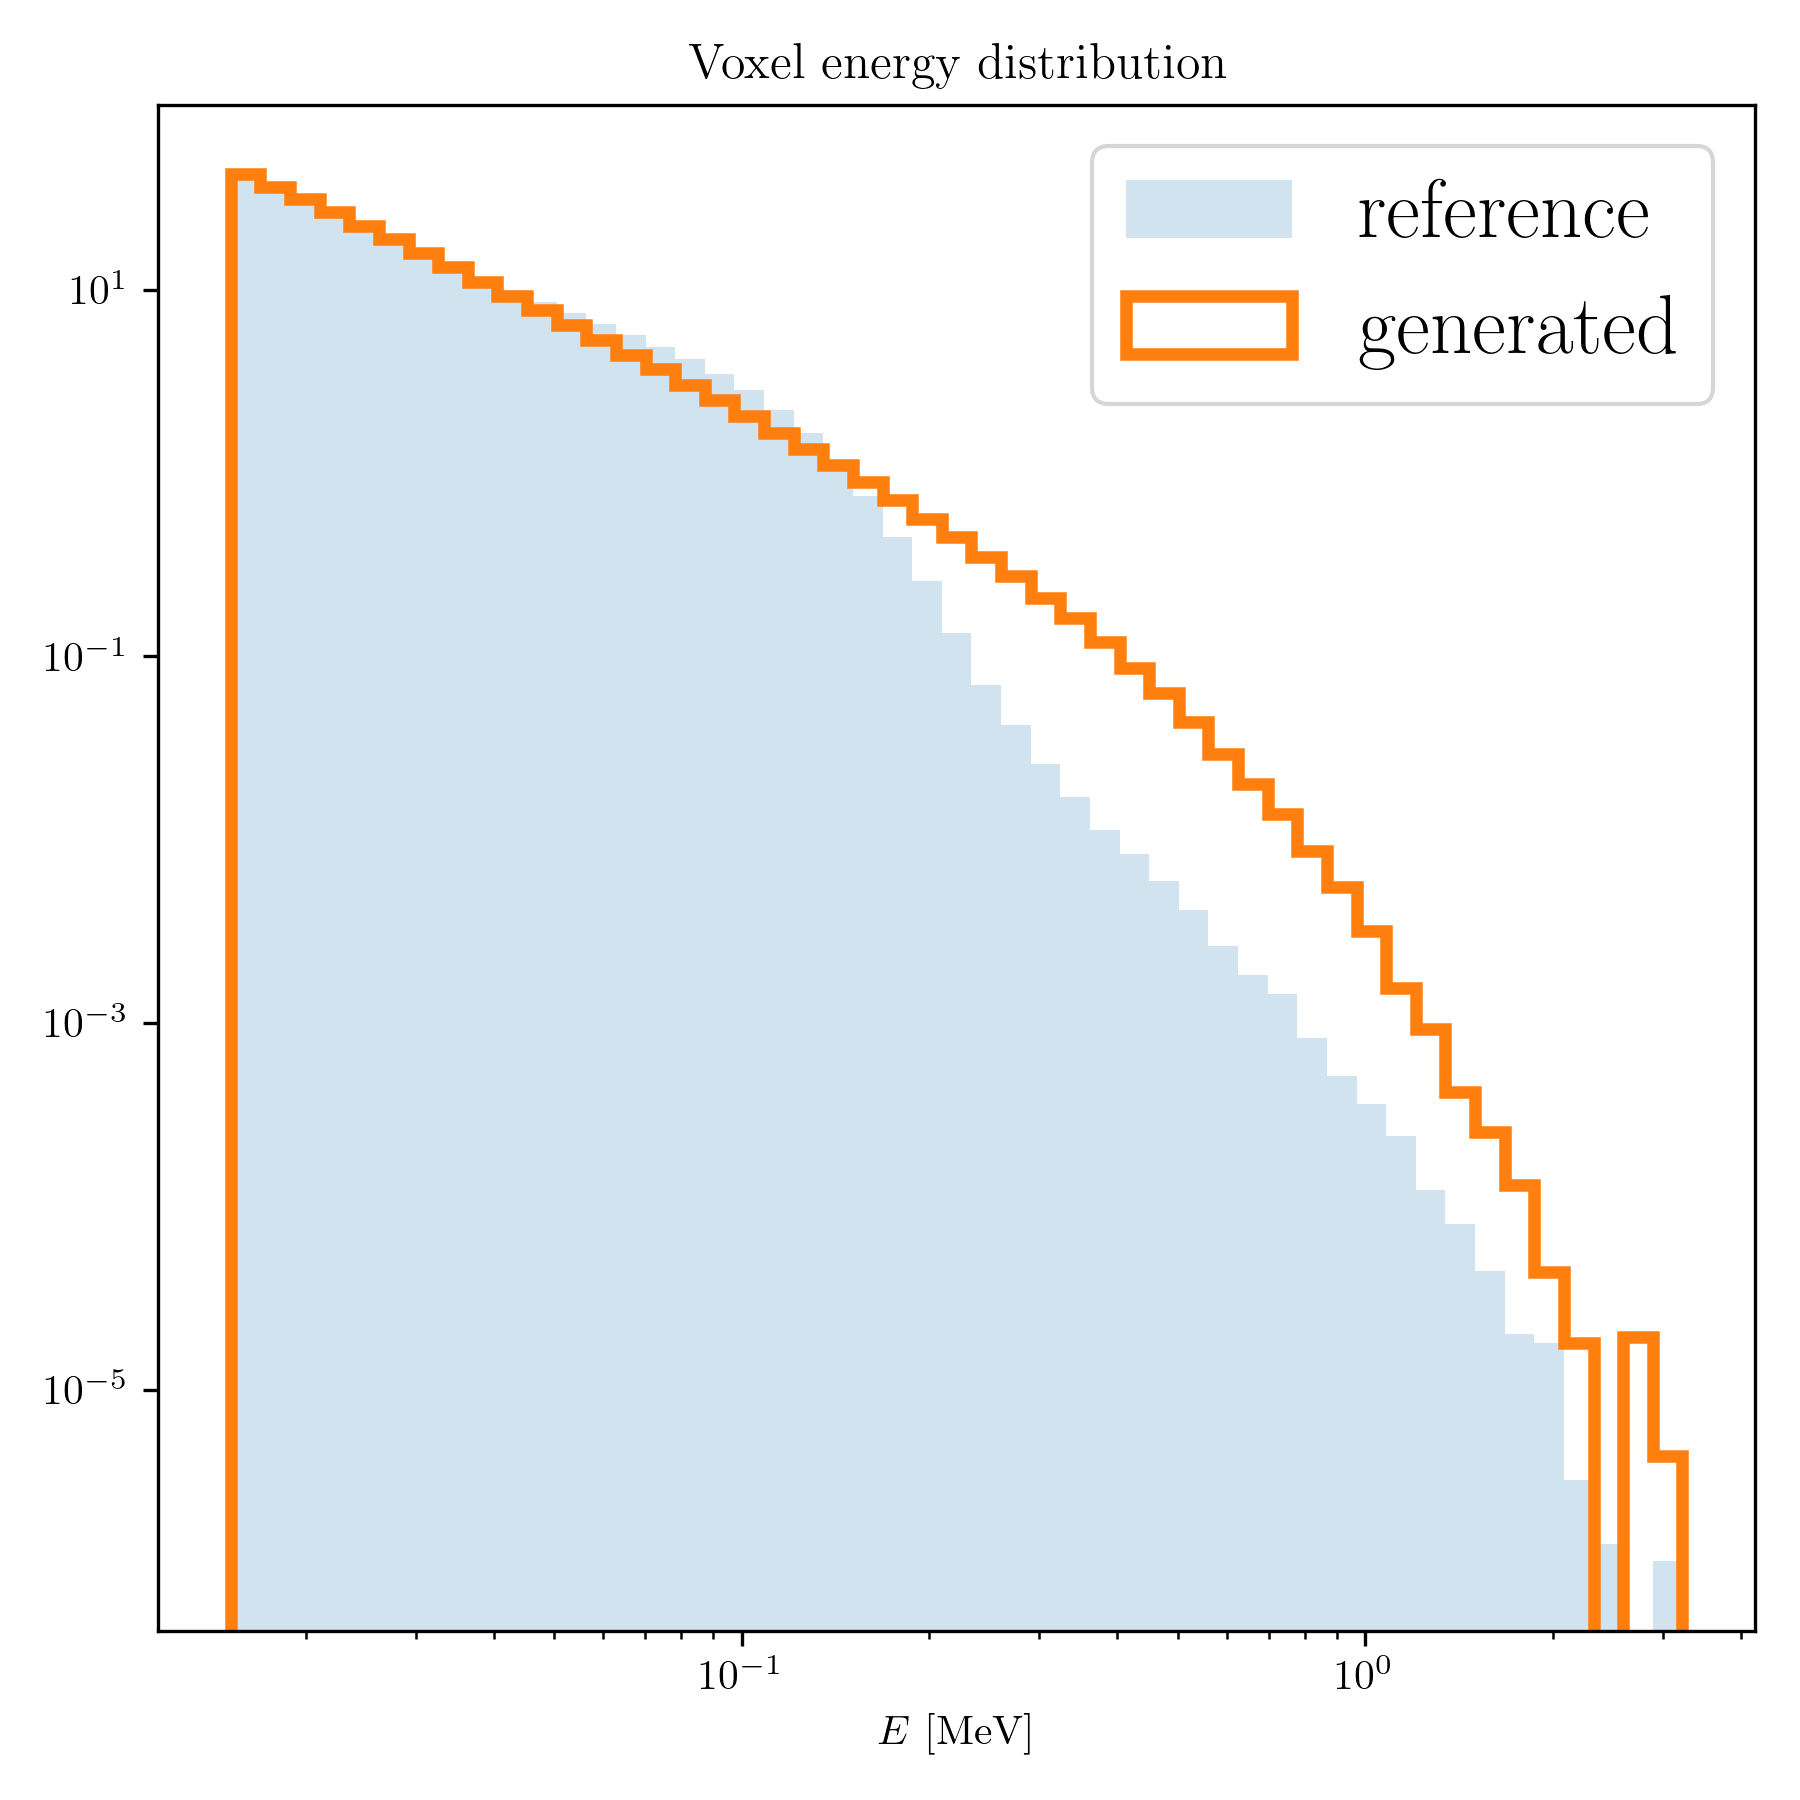
\includegraphics[width=\textwidth]{Figures/exponential6.png}
        \caption{Energy Deposit}
        \label{fig:exp6}
    \end{subfigure}
    \caption{Result for using exponential preprocessor}
\end{figure}

\newpage
\section{Result for using different SDE settings}
% every 7 pictures for VE,VP for sde =1,5,10,20. Total 7*2*4=56 pictures

\begin{figure}[bthp]
    \centering
    % First row: 4 figures
    \begin{subfigure}[b]{0.23\textwidth}
        \centering
        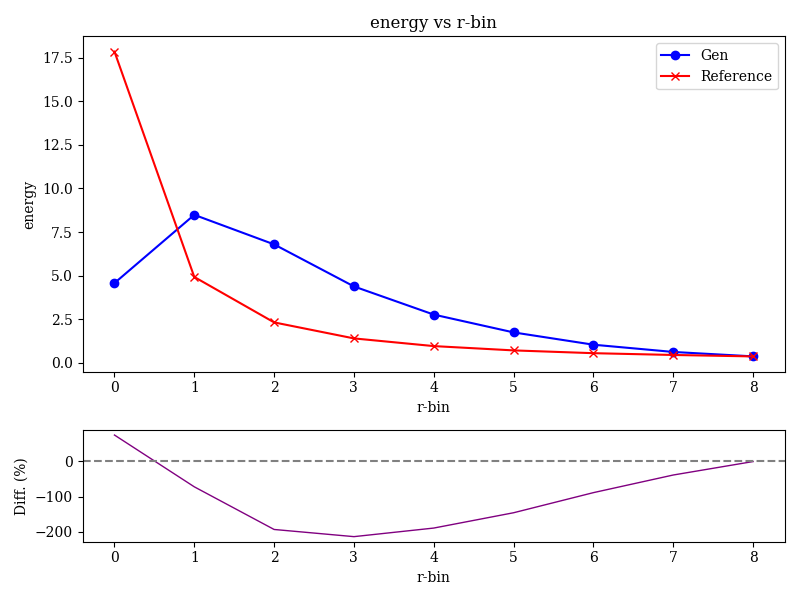
\includegraphics[width=\textwidth]{Figures/ve20_2.png}
        \caption{$\sigma_{max}=20$}
        \label{fig:ve20_2}
    \end{subfigure}
    \hfill
    \begin{subfigure}[b]{0.23\textwidth}
        \centering
        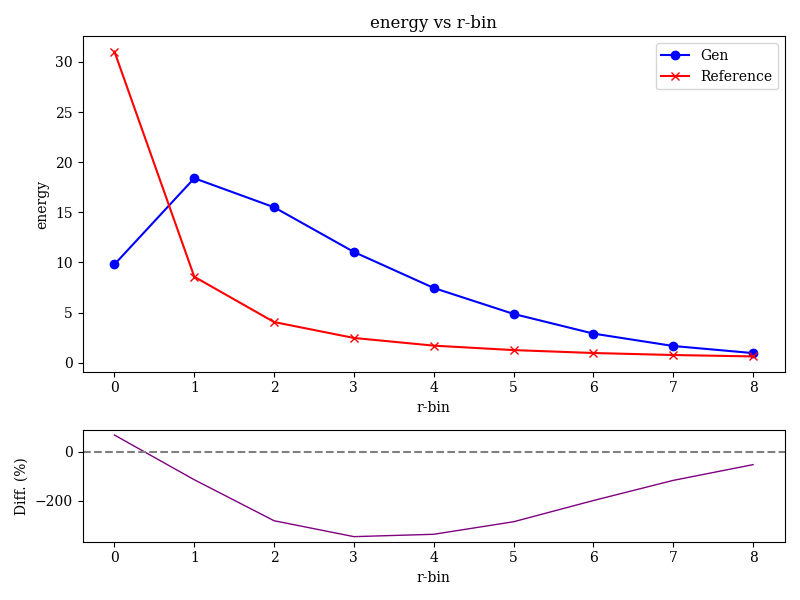
\includegraphics[width=\textwidth]{Figures/ve10_2.png}
        \caption{$\sigma_{max}=10$}
        \label{fig:ve10_2}
    \end{subfigure}
    \hfill
    \begin{subfigure}[b]{0.23\textwidth}
        \centering
        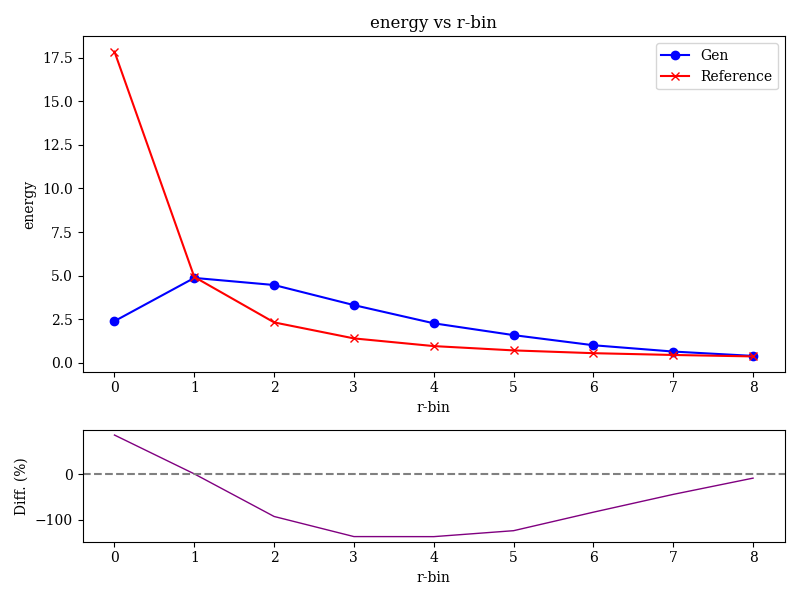
\includegraphics[width=\textwidth]{Figures/ve5_2.png}
        \caption{$\sigma_{max}=5$}
        \label{fig:ve5_2}
    \end{subfigure}
    \hfill
    \begin{subfigure}[b]{0.23\textwidth}  % Adjust width to fit 4 figures
        \centering
        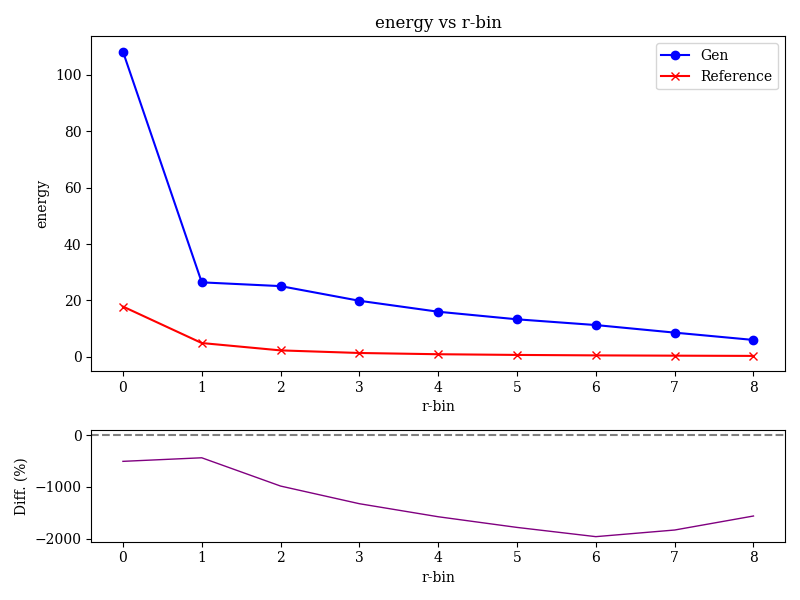
\includegraphics[width=\textwidth]{Figures/ve1_2.png}
        \caption{$\sigma_{max}=1$}
        \label{fig:ve1_2}
    \end{subfigure}
    \caption{Result for Energy vs Radius for VE}
\end{figure}

\begin{figure}[bthp]
    \centering
    % First row: 4 figures
    \begin{subfigure}[b]{0.23\textwidth}
        \centering
        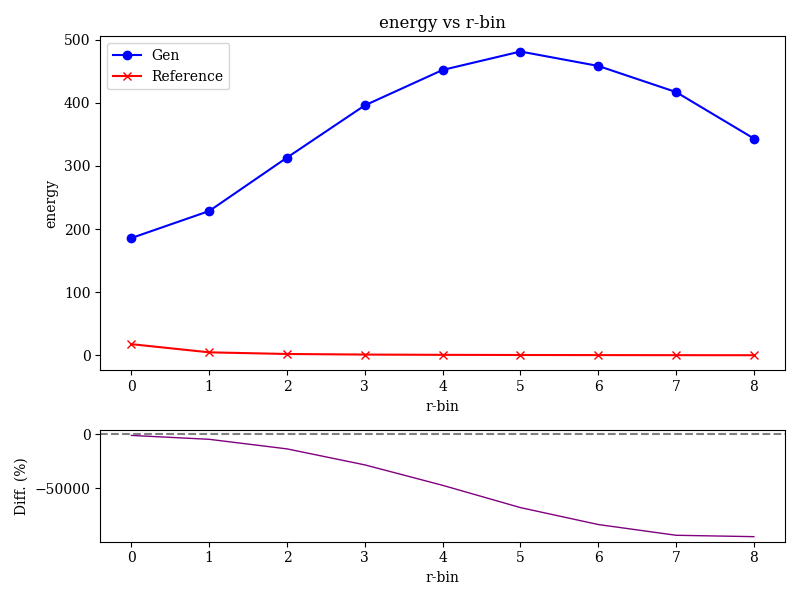
\includegraphics[width=\textwidth]{Figures/vp20_2.png}
        \caption{$\sigma_{max}=20$}
        \label{fig:vp20_2}
    \end{subfigure}
    \hfill
    \begin{subfigure}[b]{0.23\textwidth}
        \centering
        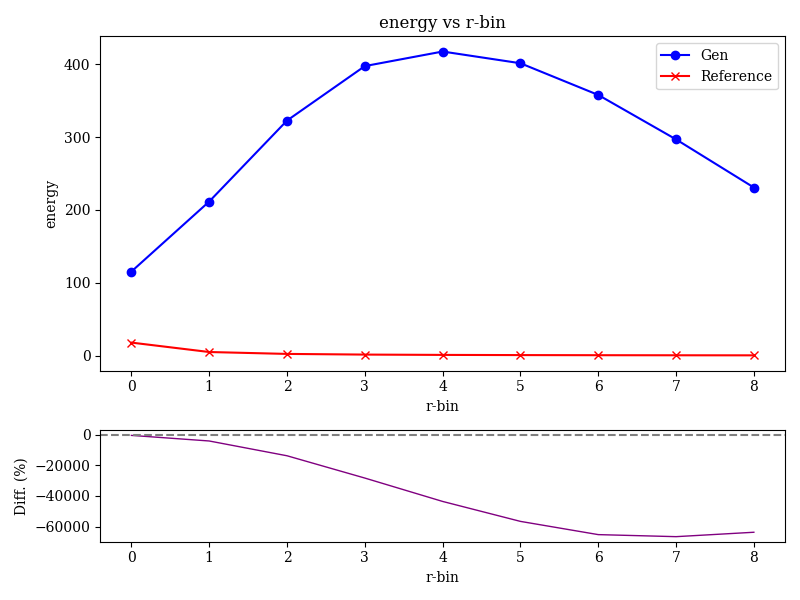
\includegraphics[width=\textwidth]{Figures/vp10_2.png}
        \caption{$\sigma_{max}=10$}
        \label{fig:vp10_2}
    \end{subfigure}
    \hfill
    \begin{subfigure}[b]{0.23\textwidth}
        \centering
        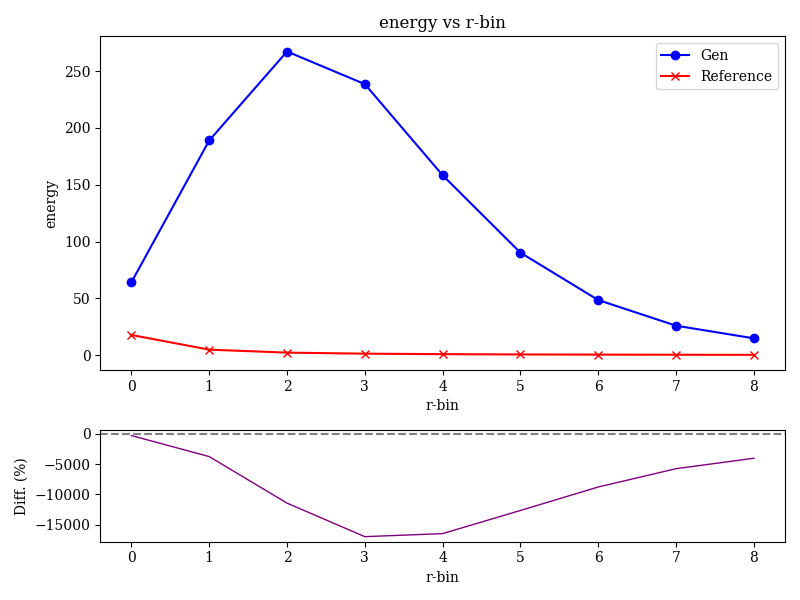
\includegraphics[width=\textwidth]{Figures/vp5_2.png}
        \caption{$\sigma_{max}=5$}
        \label{fig:vp5_2}
    \end{subfigure}
    \hfill
    \begin{subfigure}[b]{0.23\textwidth}  % Adjust width to fit 4 figures
        \centering
        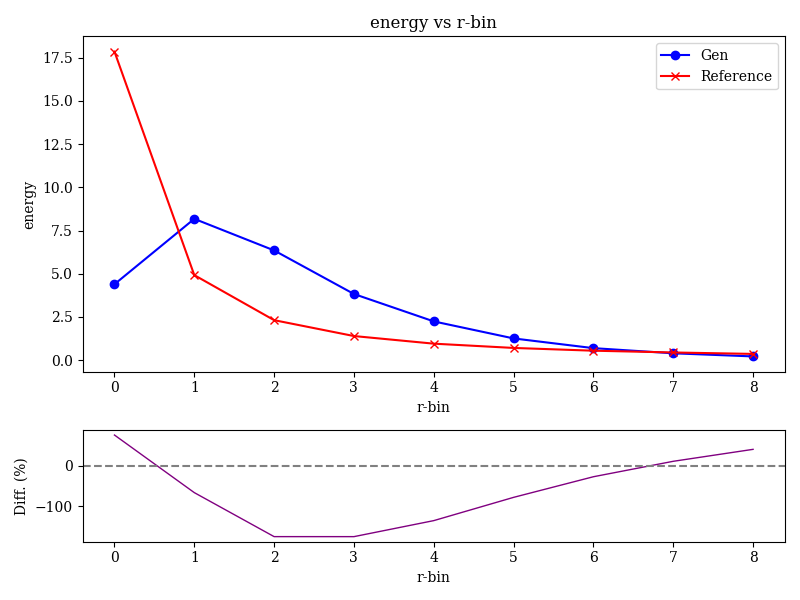
\includegraphics[width=\textwidth]{Figures/vp1_2.png}
        \caption{$\sigma_{max}=1$}
        \label{fig:vp1_2}
    \end{subfigure}
    \caption{Result for Energy vs Radius for VP}
\end{figure}

\begin{figure}[bthp]
    \centering
    % First row: 4 figures
    \begin{subfigure}[b]{0.23\textwidth}
        \centering
        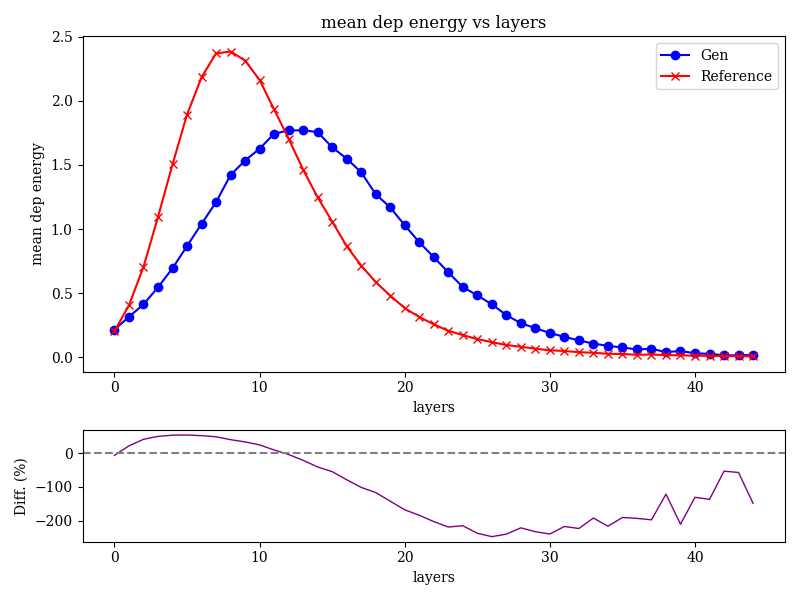
\includegraphics[width=\textwidth]{Figures/ve20_3.png}
        \caption{$\sigma_{max}=20$}
        \label{fig:ve20_3}
    \end{subfigure}
    \hfill
    \begin{subfigure}[b]{0.23\textwidth}
        \centering
        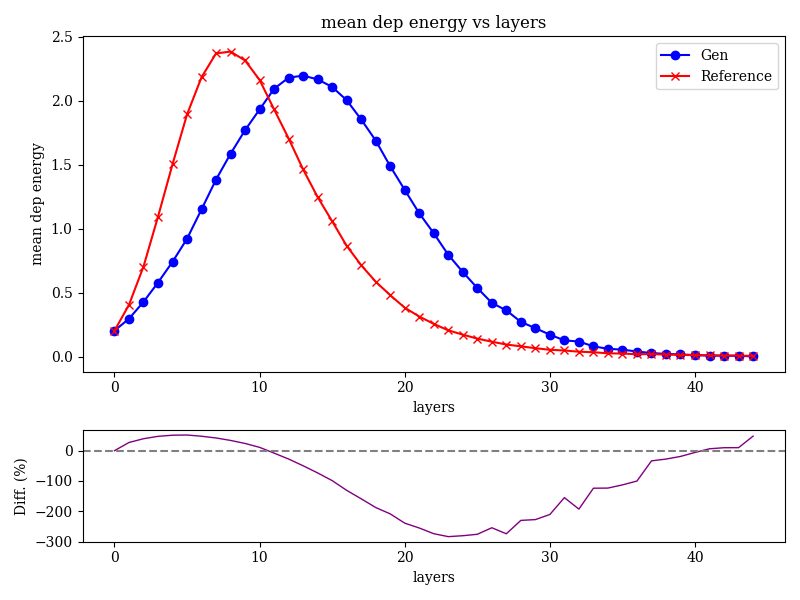
\includegraphics[width=\textwidth]{Figures/ve10_3.png}
        \caption{$\sigma_{max}=10$}
        \label{fig:ve10_3}
    \end{subfigure}
    \hfill
    \begin{subfigure}[b]{0.23\textwidth}
        \centering
        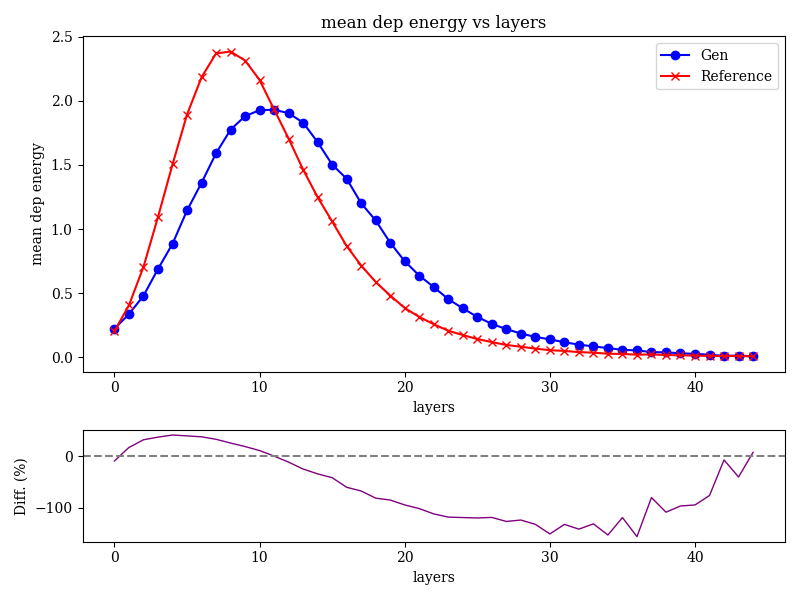
\includegraphics[width=\textwidth]{Figures/ve5_3.png}
        \caption{$\sigma_{max}=5$}
        \label{fig:ve5_3}
    \end{subfigure}
    \hfill
    \begin{subfigure}[b]{0.23\textwidth}  % Adjust width to fit 4 figures
        \centering
        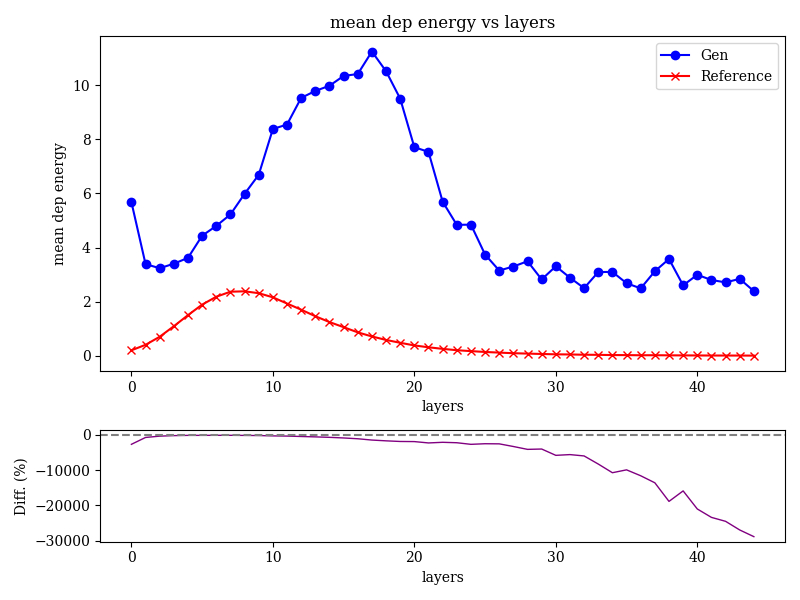
\includegraphics[width=\textwidth]{Figures/ve1_3.png}
        \caption{$\sigma_{max}=1$}
        \label{fig:ve1_3}
    \end{subfigure}
    \caption{Result for Energy vs Layers for VE}
\end{figure}

\begin{figure}[bthp]
    \centering
    % First row: 4 figures
    \begin{subfigure}[b]{0.23\textwidth}
        \centering
        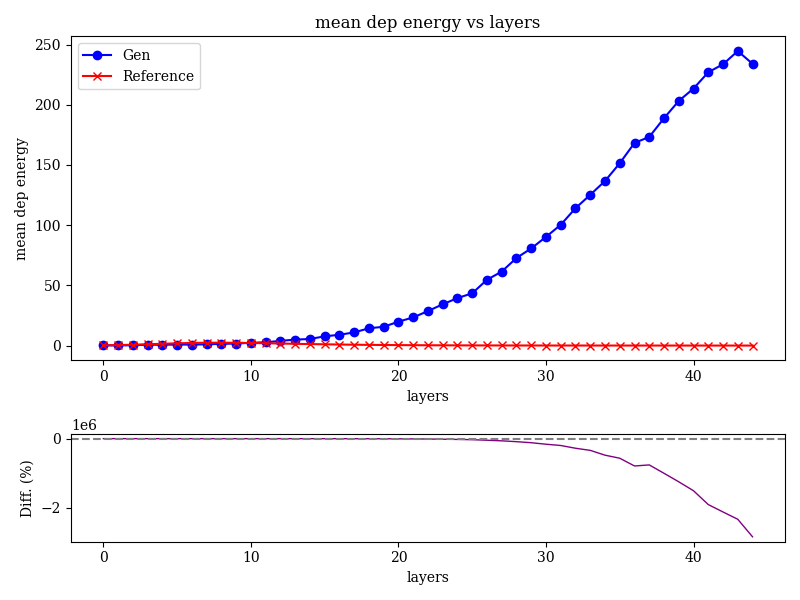
\includegraphics[width=\textwidth]{Figures/vp20_3.png}
        \caption{$\sigma_{max}=20$}
        \label{fig:vp20_3}
    \end{subfigure}
    \hfill
    \begin{subfigure}[b]{0.23\textwidth}
        \centering
        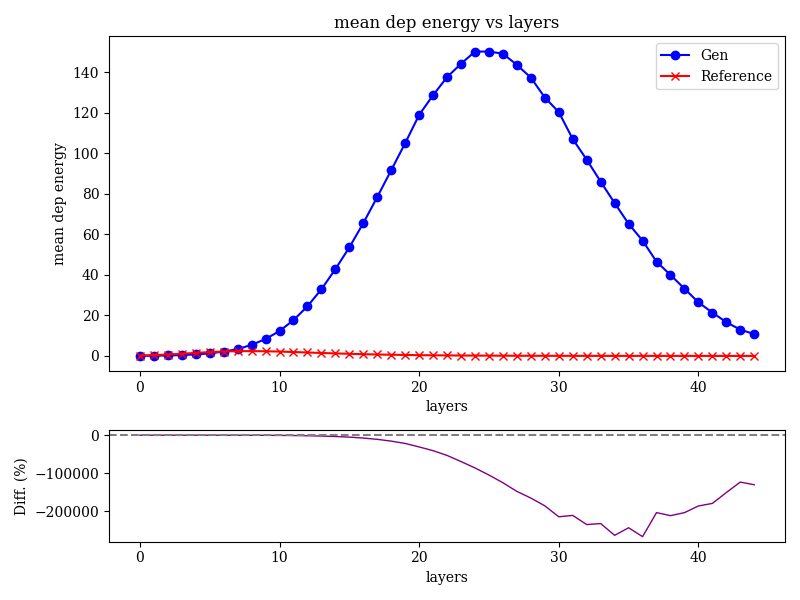
\includegraphics[width=\textwidth]{Figures/vp10_3.png}
        \caption{$\sigma_{max}=10$}
        \label{fig:vp10_3}
    \end{subfigure}
    \hfill
    \begin{subfigure}[b]{0.23\textwidth}
        \centering
        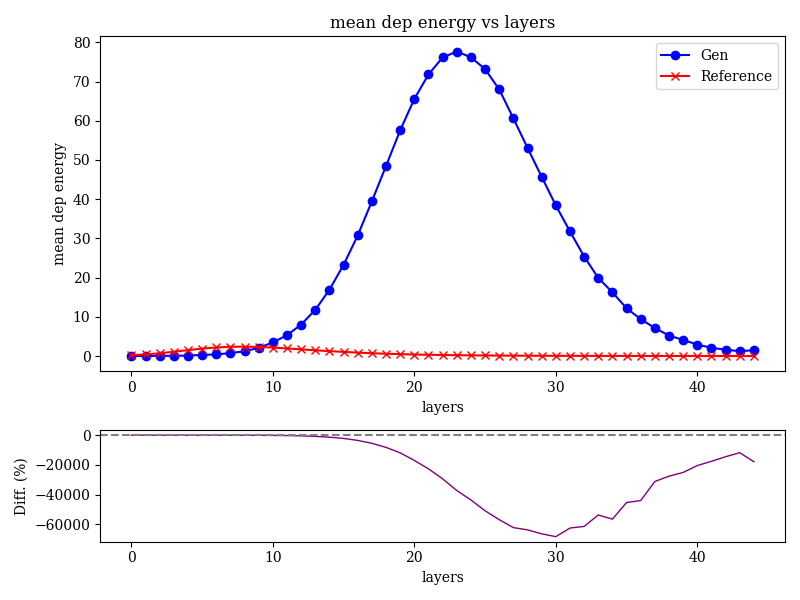
\includegraphics[width=\textwidth]{Figures/vp5_3.png}
        \caption{$\sigma_{max}=5$}
        \label{fig:vp5_3}
    \end{subfigure}
    \hfill
    \begin{subfigure}[b]{0.23\textwidth}  % Adjust width to fit 4 figures
        \centering
        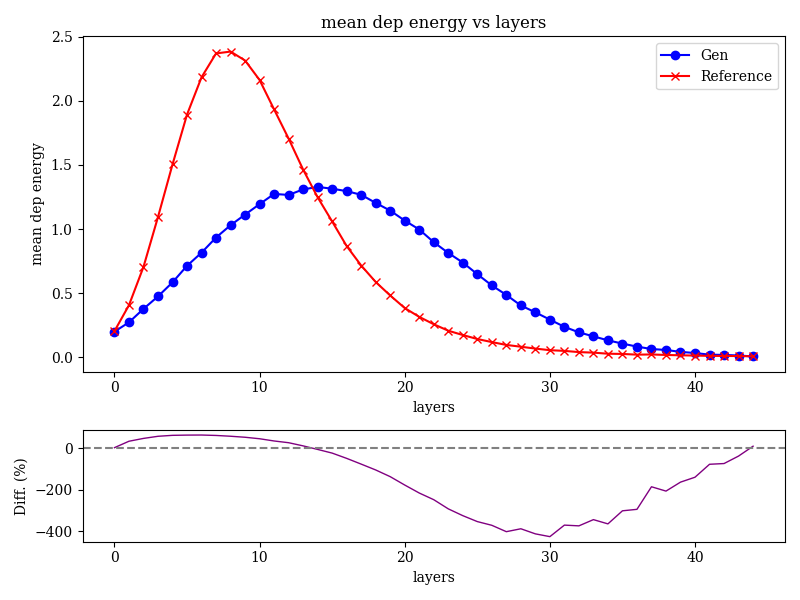
\includegraphics[width=\textwidth]{Figures/vp1_3.png}
        \caption{$\sigma_{max}=1$}
        \label{fig:vp1_3}
    \end{subfigure}
    \caption{Result for Energy vs Layers for VP}
\end{figure}

\begin{figure}[bthp]
    \centering
    % First row: 4 figures
    \begin{subfigure}[b]{0.23\textwidth}
        \centering
        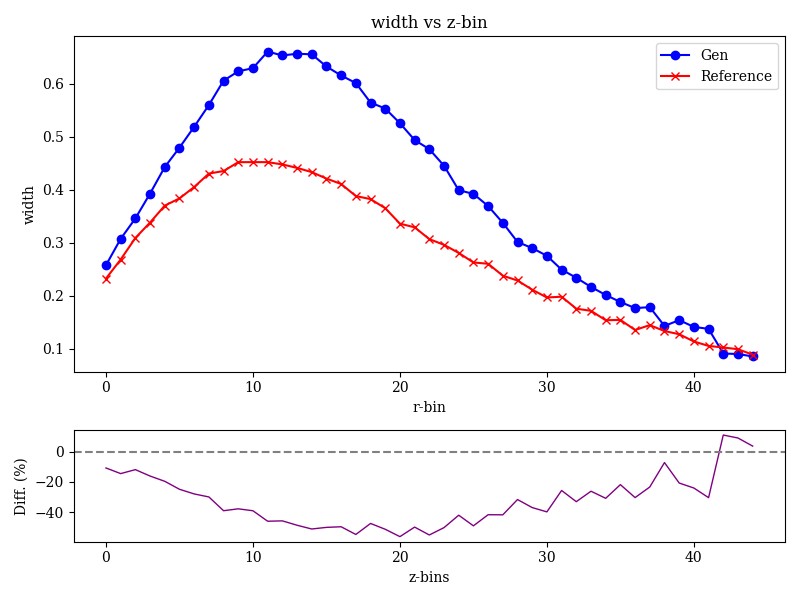
\includegraphics[width=\textwidth]{Figures/ve20_4.png}
        \caption{$\sigma_{max}=20$}
        \label{fig:ve20_4}
    \end{subfigure}
    \hfill
    \begin{subfigure}[b]{0.23\textwidth}
        \centering
        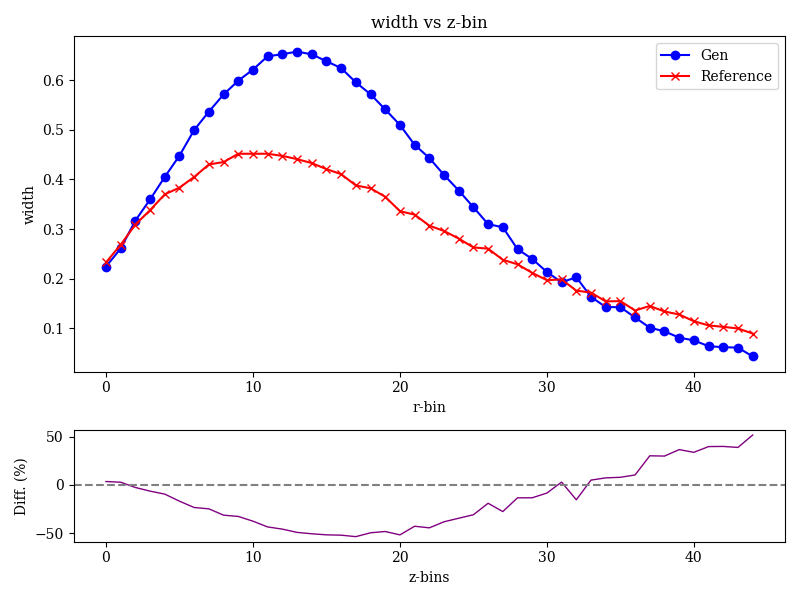
\includegraphics[width=\textwidth]{Figures/ve10_4.png}
        \caption{$\sigma_{max}=10$}
        \label{fig:ve10_4}
    \end{subfigure}
    \hfill
    \begin{subfigure}[b]{0.23\textwidth}
        \centering
        \includegraphics[width=\textwidth]{Figures/ve5_4.png}
        \caption{$\sigma_{max}=5$}
        \label{fig:ve5_4}
    \end{subfigure}
    \hfill
    \begin{subfigure}[b]{0.23\textwidth}  % Adjust width to fit 4 figures
        \centering
        \includegraphics[width=\textwidth]{Figures/ve1_4.png}
        \caption{$\sigma_{max}=1$}
        \label{fig:ve1_4}
    \end{subfigure}
    \caption{Result for R-width vs Layers for VE}
\end{figure}

\begin{figure}[bthp]
    \centering
    % First row: 4 figures
    \begin{subfigure}[b]{0.23\textwidth}
        \centering
        \includegraphics[width=\textwidth]{Figures/vp20_4.png}
        \caption{$\sigma_{max}=20$}
        \label{fig:vp20_4}
    \end{subfigure}
    \hfill
    \begin{subfigure}[b]{0.23\textwidth}
        \centering
        \includegraphics[width=\textwidth]{Figures/vp10_4.png}
        \caption{$\sigma_{max}=10$}
        \label{fig:vp10_4}
    \end{subfigure}
    \hfill
    \begin{subfigure}[b]{0.23\textwidth}
        \centering
        \includegraphics[width=\textwidth]{Figures/vp5_4.png}
        \caption{$\sigma_{max}=5$}
        \label{fig:vp5_4}
    \end{subfigure}
    \hfill
    \begin{subfigure}[b]{0.23\textwidth}  % Adjust width to fit 4 figures
        \centering
        \includegraphics[width=\textwidth]{Figures/vp1_4.png}
        \caption{$\sigma_{max}=1$}
        \label{fig:vp1_4}
    \end{subfigure}
    \caption{Result for R-width vs Layers for VP}
\end{figure}

\begin{figure}[bthp]
    \centering
    % First row: 4 figures
    \begin{subfigure}[b]{0.23\textwidth}
        \centering
        \includegraphics[width=\textwidth]{Figures/ve20_5.png}
        \caption{$\sigma_{max}=20$}
        \label{fig:ve20_5}
    \end{subfigure}
    \hfill
    \begin{subfigure}[b]{0.23\textwidth}
        \centering
        \includegraphics[width=\textwidth]{Figures/ve10_5.png}
        \caption{$\sigma_{max}=10$}
        \label{fig:ve10_5}
    \end{subfigure}
    \hfill
    \begin{subfigure}[b]{0.23\textwidth}
        \centering
        \includegraphics[width=\textwidth]{Figures/ve5_5.png}
        \caption{$\sigma_{max}=5$}
        \label{fig:ve5_5}
    \end{subfigure}
    \hfill
    \begin{subfigure}[b]{0.23\textwidth}  % Adjust width to fit 4 figures
        \centering
        \includegraphics[width=\textwidth]{Figures/ve1_5.png}
        \caption{$\sigma_{max}=1$}
        \label{fig:ve1_5}
    \end{subfigure}
    \caption{Result for Max Voxel Deposit vs Layer for VE}
\end{figure}

\begin{figure}
    \centering
    % First row: 4 figures
    \begin{subfigure}[b]{0.23\textwidth}
        \centering
        \includegraphics[width=\textwidth]{Figures/vp20_5.png}
        \caption{$\sigma_{max}=20$}
        \label{fig:vp20_5}
    \end{subfigure}
    \hfill
    \begin{subfigure}[b]{0.23\textwidth}
        \centering
        \includegraphics[width=\textwidth]{Figures/vp10_5.png}
        \caption{$\sigma_{max}=10$}
        \label{fig:vp10_5}
    \end{subfigure}
    \hfill
    \begin{subfigure}[b]{0.23\textwidth}
        \centering
        \includegraphics[width=\textwidth]{Figures/vp5_5.png}
        \caption{$\sigma_{max}=5$}
        \label{fig:vp5_5}
    \end{subfigure}
    \hfill
    \begin{subfigure}[b]{0.23\textwidth}  % Adjust width to fit 4 figures
        \centering
        \includegraphics[width=\textwidth]{Figures/vp1_5.png}
        \caption{$\sigma_{max}=1$}
        \label{fig:vp1_5}
    \end{subfigure}
    \caption{Result for Max Voxel Deposit vs Layer for VP}
\end{figure}

\begin{figure}
    \centering
    % First row: 4 figures
    \begin{subfigure}[b]{0.23\textwidth}
        \centering
        \includegraphics[width=\textwidth]{Figures/ve20_1dpng.png}
        \caption{$\sigma_{max}=20$}
        \label{fig:ve20_1}
    \end{subfigure}
    \hfill
    \begin{subfigure}[b]{0.23\textwidth}
        \centering
        \includegraphics[width=\textwidth]{Figures/ve10_1.png}
        \caption{$\sigma_{max}=10$}
        \label{fig:ve10_1}
    \end{subfigure}
    \hfill
    \begin{subfigure}[b]{0.23\textwidth}
        \centering
        \includegraphics[width=\textwidth]{Figures/ve5_1.png}
        \caption{$\sigma_{max}=5$}
        \label{fig:ve5_1}
    \end{subfigure}
    \hfill
    \begin{subfigure}[b]{0.23\textwidth}  % Adjust width to fit 4 figures
        \centering
        \includegraphics[width=\textwidth]{Figures/ve1_1.png}
        \caption{$\sigma_{max}=1$}
        \label{fig:ve1_1}
    \end{subfigure}
    \caption{Result for Each Dimension VE}
\end{figure}

\begin{figure}
    \centering
    % First row: 4 figures
    \begin{subfigure}[b]{0.23\textwidth}
        \centering
        \includegraphics[width=\textwidth]{Figures/vp20_1.png}
        \caption{$\sigma_{max}=20$}
        \label{fig:vp20_1}
    \end{subfigure}
    \hfill
    \begin{subfigure}[b]{0.23\textwidth}
        \centering
        \includegraphics[width=\textwidth]{Figures/vp10_1.png}
        \caption{$\sigma_{max}=10$}
        \label{fig:vp10_1}
    \end{subfigure}
    \hfill
    \begin{subfigure}[b]{0.23\textwidth}
        \centering
        \includegraphics[width=\textwidth]{Figures/vp5_1.png}
        \caption{$\sigma_{max}=5$}
        \label{fig:vp5_1}
    \end{subfigure}
    \hfill
    \begin{subfigure}[b]{0.23\textwidth}  % Adjust width to fit 4 figures
        \centering
        \includegraphics[width=\textwidth]{Figures/vp1_1.png}
        \caption{$\sigma_{max}=1$}
        \label{fig:vp1_1}
    \end{subfigure}
    \caption{Result for Each Dimension VP}
\end{figure}

\begin{figure}
    \centering
    % First row: 4 figures
    \begin{subfigure}[b]{0.23\textwidth}
        \centering
        \includegraphics[width=\textwidth]{Figures/ve20_6.png}
        \caption{$\sigma_{max}=20$}
        \label{fig:ve20_6}
    \end{subfigure}
    \hfill
    \begin{subfigure}[b]{0.23\textwidth}
        \centering
        \includegraphics[width=\textwidth]{Figures/ve10_6.png}
        \caption{$\sigma_{max}=10$}
        \label{fig:ve10_6}
    \end{subfigure}
    \hfill
    \begin{subfigure}[b]{0.23\textwidth}
        \centering
        \includegraphics[width=\textwidth]{Figures/ve5_6.png}
        \caption{$\sigma_{max}=5$}
        \label{fig:ve5_6}
    \end{subfigure}
    \hfill
    \begin{subfigure}[b]{0.23\textwidth}  % Adjust width to fit 4 figures
        \centering
        \includegraphics[width=\textwidth]{Figures/ve1_6.png}
        \caption{$\sigma_{max}=1$}
        \label{fig:ve1_6}
    \end{subfigure}
    \caption{Result for Energy Voxel Comparison for VE}
\end{figure}

\begin{figure}
    \centering
    % First row: 4 figures
    \begin{subfigure}[b]{0.23\textwidth}
        \centering
        \includegraphics[width=\textwidth]{Figures/vp20_6.png}
        \caption{$\sigma_{max}=20$}
        \label{fig:vp20_6}
    \end{subfigure}
    \hfill
    \begin{subfigure}[b]{0.23\textwidth}
        \centering
        \includegraphics[width=\textwidth]{Figures/vp10_6.png}
        \caption{$\sigma_{max}=10$}
        \label{fig:vp10_6}
    \end{subfigure}
    \hfill
    \begin{subfigure}[b]{0.23\textwidth}
        \centering
        \includegraphics[width=\textwidth]{Figures/vp5_6.png}
        \caption{$\sigma_{max}=5$}
        \label{fig:vp5_6}
    \end{subfigure}
    \hfill
    \begin{subfigure}[b]{0.23\textwidth}  % Adjust width to fit 4 figures
        \centering
        \includegraphics[width=\textwidth]{Figures/vp1_6.png}
        \caption{$\sigma_{max}=1$}
        \label{fig:vp1_6}
    \end{subfigure}
    \caption{Result for Energy Voxel Comparison for VP}
\end{figure}

\begin{figure}
    \centering
    % First row: 4 figures
    \begin{subfigure}[b]{0.23\textwidth}
        \centering
        \includegraphics[width=\textwidth]{Figures/ve20_7.png}
        \caption{$\sigma_{max}=20$}
        \label{fig:ve20_7}
    \end{subfigure}
    \hfill
    \begin{subfigure}[b]{0.23\textwidth}
        \centering
        \includegraphics[width=\textwidth]{Figures/ve10_7.png}
        \caption{$\sigma_{max}=10$}
        \label{fig:ve10_7}
    \end{subfigure}
    \hfill
    \begin{subfigure}[b]{0.23\textwidth}
        \centering
        \includegraphics[width=\textwidth]{Figures/ve5_7.png}
        \caption{$\sigma_{max}=5$}
        \label{fig:ve5_7}
    \end{subfigure}
    \hfill
    \begin{subfigure}[b]{0.23\textwidth}  % Adjust width to fit 4 figures
        \centering
        \includegraphics[width=\textwidth]{Figures/ve1_7.png}
        \caption{$\sigma_{max}=1$}
        \label{fig:ve1_7}
    \end{subfigure}
    \caption{Result for Energy Deposit for VE}
\end{figure}

\begin{figure}
    \centering
    % First row: 4 figures
    \begin{subfigure}[b]{0.23\textwidth}
        \centering
        \includegraphics[width=\textwidth]{Figures/vp20_7.png}
        \caption{$\sigma_{max}=20$}
        \label{fig:vp20_7}
    \end{subfigure}
    \hfill
    \begin{subfigure}[b]{0.23\textwidth}
        \centering
        \includegraphics[width=\textwidth]{Figures/vp10_7.png}
        \caption{$\sigma_{max}=10$}
        \label{fig:vp10_7}
    \end{subfigure}
    \hfill
    \begin{subfigure}[b]{0.23\textwidth}
        \centering
        \includegraphics[width=\textwidth]{Figures/vp5_7.png}
        \caption{$\sigma_{max}=5$}
        \label{fig:vp5_7}
    \end{subfigure}
    \hfill
    \begin{subfigure}[b]{0.23\textwidth}  % Adjust width to fit 4 figures
        \centering
        \includegraphics[width=\textwidth]{Figures/vp1_7.png}
        \caption{$\sigma_{max}=1$}
        \label{fig:vp1_7}
    \end{subfigure}
    \caption{Result for Energy Deposit for VP}
\end{figure}